% ---------------------------------------------------------------------------------------------------------------
\Chapter{Charge monitoring}{The ATLAS Diamond Beam Monitor}
%\chapter{Charge monitoring}
% ---------------------------------------------------------------------------------------------------------------




Particle detectors in high energy physics experiments need to meet very stringent specifications, depending on the functionality and their position in the experiment. In particular, the detectors close to the collision point are subject to high levels of radiation. In addition, they need to operate with a high spatial and temporal segmentation to be able to precisely measure trajectories of hundreds of particles in very short time. In addition, they need to be highly efficient. In terms of the structure, their active sensing material has to be thin so as not to cause the particles to scatter or get stopped, which would worsen the measurements. This also means that they have to have a low heat dissipation so that the cooling system dimensions can be minimised. Finally, they need to be able to have a stable operation for several years without a required intervention, because they are buried deep under tonnes of material and electronics. 

The material of choice for the inner detector layers in the HEP experiments is silicon. It can withstand high doses of radiation, it is highly efficient (of the order of $\sim$99.9~\%) and relatively low cost due to using existing industrial processes for its production. Its downside is that, with increasing irradiation levels, it needs to be cooled to increasingly low temperatures to ensure a stable operation. This is not the case with diamond. In addition, diamond has a lower radiation damage factor, which means it can operate in a radiation-heavy environment for a longer period.

The ATLAS Diamond Beam Monitor (the DBM)~\cite{Cerv:1630832} is a novel high energy charged particle detector. Its function is to measure luminosity and beam background in the ATLAS experiment. Given its position in a region with a high radiation dose, diamond was chosen as the sensing material. The monitor's pCVD diamond sensors are instrumented with pixellated FE-I4 front-end chips. The pCVD diamond sensor material was chosen to ensure the durability of the sensors in a radiation-hard environment and the size of its active area. The DBM is not the first diamond detector used in HEP, but it is the largest pixellated detector installed thus far, as shown in figure~\ref{fig:areavsyear}. It was designed as an upgrade to the existing luminosity monitor called the Beam Conditions Monitor (BCM)~\cite{Gorisek:1062633} consisting of eight diamond pad detectors. The BCM is able to perform precise time-of-flight (ToF) measurements. The DBM complements the BCM's features by implementing tracking capability. Its pixelated front-end electronics significantly increase the spatial resolution of the system. Furthermore, the DBM is able to distinguish particle tracks originating in the collision region from the background hits. This capability is a result of its projective geometry pointing towards the interaction region. This chapter first describes the principles of luminosity measurements. It then explains how the DBM carries out this task. Finally, some results from the commissioning and from the real collisions are presented. 

When a particle traverses a sensor plane, a hit is recorded in the corresponding pixel. Thus, a precise spatial and timing information of the hit is extracted. With three or more sensors stacked behind each other, it is also possible to define the particle's trajectory. This is the case with the DBM. Its projective geometry allows the particles to be tracked if they traverse the sensor planes. The DBM relates the luminosity to the number of particle tracks that originate from the collision region of the ATLAS experiment. Particles that hit the DBM from other directions are rejected as background radiation.

\begin{figure}[!t]
\centering
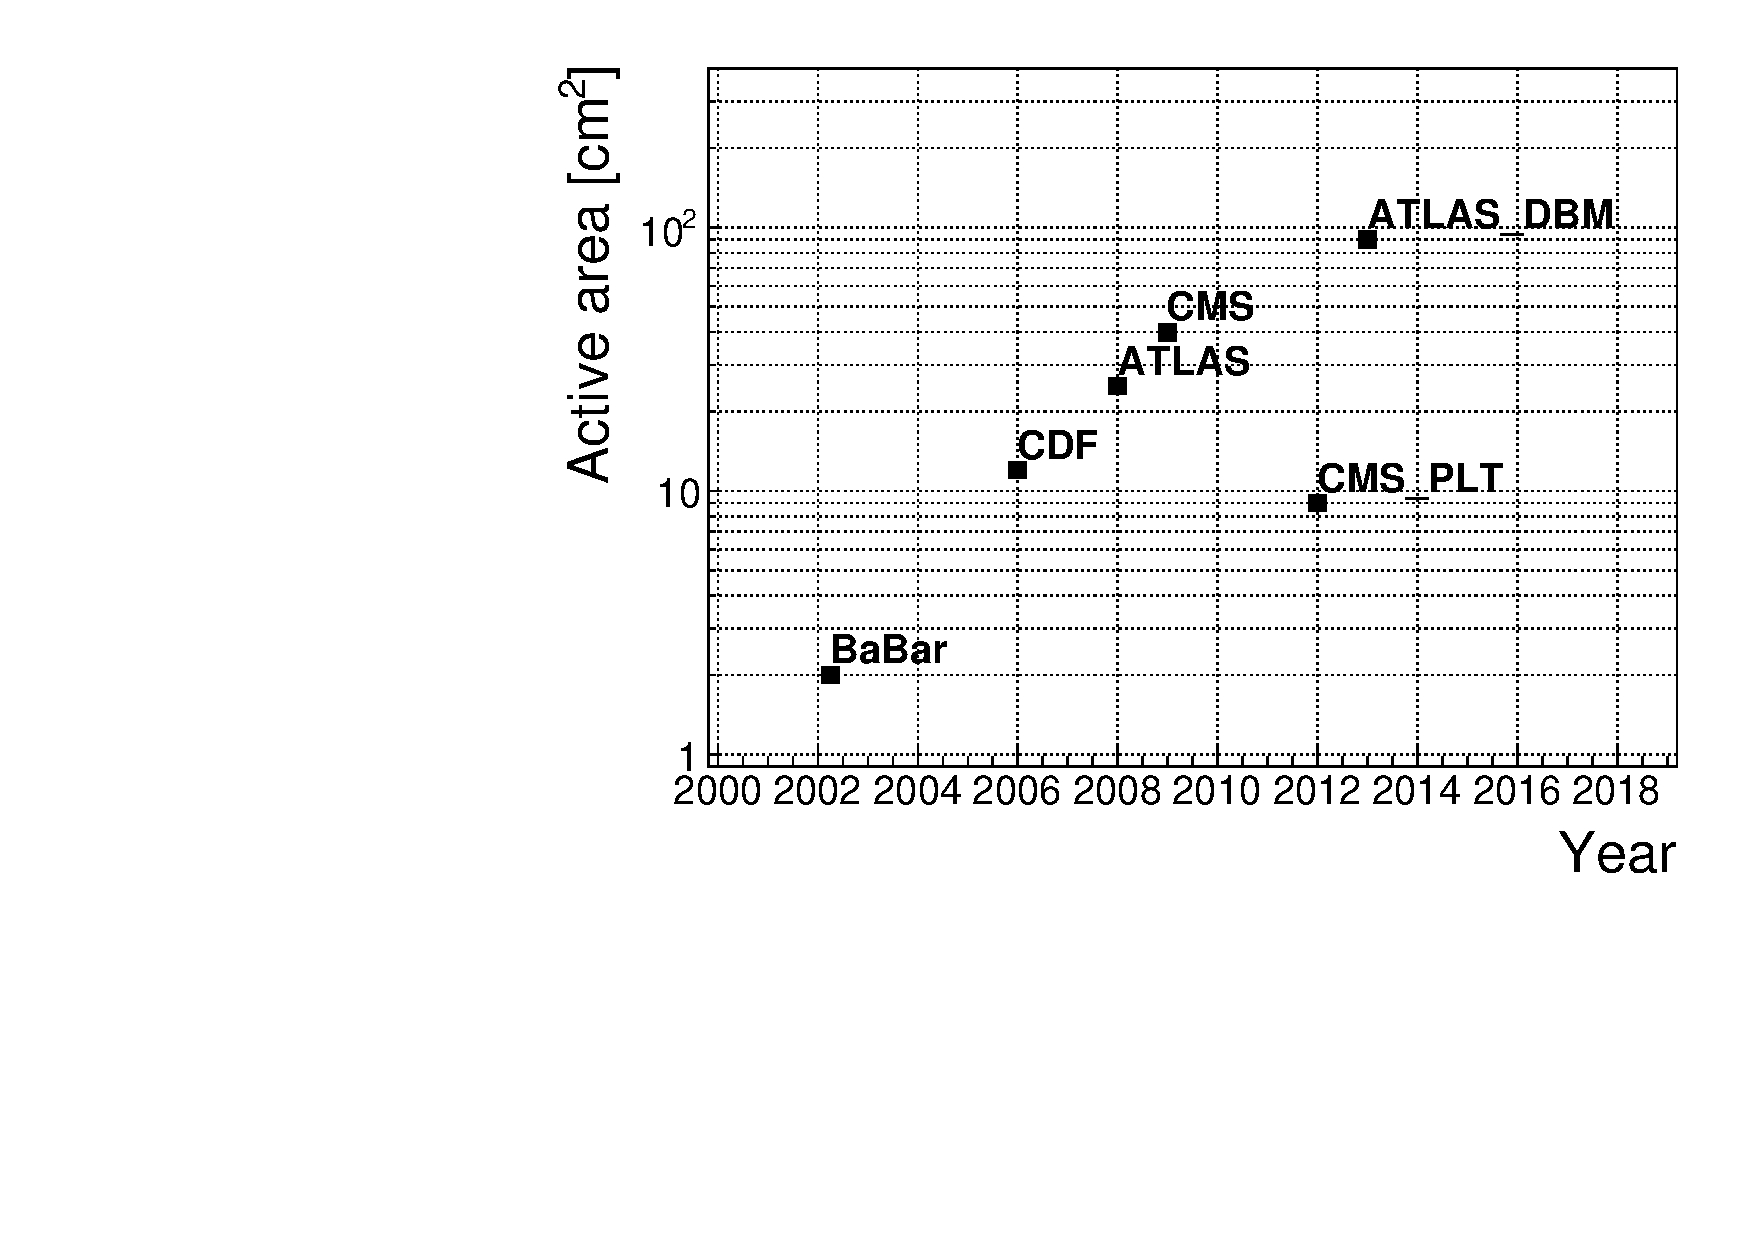
\includegraphics[width=0.7\textwidth]{../scripts/04_charge_monitoring/plots/detArea}
\caption{Diamond detectors installed in high-energy physics experiments in the last decade, sorted by the active sensor area. The first four detectors from the left are radiation monitors whereas the right two are pixel trackers.}
\label{fig:areavsyear}
\end{figure}

%---------------------------------------------------------------------------------------------------------------
%\clearpage
\section{Luminosity measurements}
\label{sec:lummeas}
%---------------------------------------------------------------------------------------------------------------
 \label{sec:lumi}
Luminosity is one of the most important parameters of a particle collider. It is a measurement of the rate of particle collisions that are produced by two particle beams. It can be described as a function of the beam parameters, such as: the number of colliding bunch pairs, the revolution frequency, the number of particles in each bunch and the transverse bunch dimensions. The first four parameters are well defined. However, the transverse bunch dimensions have to be determined experimentally during calibration measurements. The ATLAS experiment uses the \emph{van der Meer scan}~\cite{ATLAS-CONF-2010-102} during low-luminosity runs to calibrate the luminosity detectors. This scan is performed by displacing one beam in a given direction and measuring the rate of interactions as a function of the displacement. The transverse charge density of the bunches can be estimated on the basis of the interaction rate. The calibrated luminosity detectors can then operate during high-luminosity runs.

One approach to luminosity monitoring is to count the number of particles produced by the collisions. The luminosity is then proportional to the number of detected particles. A detector has to be capable of distinguishing individual particles that fly from the interaction point through the active sensor area. If the detector has at least three layers, it can reconstruct the particles' tracks, which in turn yields more information on the their trajectory. This is one reason why detectors with a high timing- and spatial segmentation are more suitable for these applications. The second reason is that, with a high spatial segmentation, the detector does not saturate even at high particle fluencies.





%---------------------------------------------------------------------------------------------------------------
%\clearpage
\section{Diamond pixel module}
\label{sec:atlasdbm}
%---------------------------------------------------------------------------------------------------------------
The two most important parts of the diamond pixel module are the sensor, which translates the incident ionising radiation into charge carriers as explained in chapter~\ref{ch:diamond}, and the pixellated front-end chip, which collects the ionised charge with a high spatial segmentation, processes the recorded data and sends them to the readout system. This section describes these two parts of the module and their interconnection.

\subsection{Sensors}
The DBM modules are instrumented with two types of sensors -- pCVD diamond and silicon. The silicon sensors are used as a fallback solution because there were not enough high-quality diamond sensors available during the construction phase. In addition, a comparative study of irradiation damage between silicon and diamond can be made with such a hybrid system.

 
\begin{description}
\item[Diamond sensors] The target material for this application is pCVD diamond. The reason for this is that the active area of an individual sensor must be approximately 4~cm$^2$, which is too large for the sCVD diamond. pCVD material is also a bit cheaper, which makes a detector with a large active area more feasible to build. The material is provided by three companies: DDL, E6 and II-IV and it is grown in 15~cm wafers, as seen in figure~\ref{fig:wafer}. The target thickness of the wafers is 500~$\upmu$m. The minimum required charge collection efficiency is 40~\% (CCD $\geq$ 200~um) to ensure that the MPV of the collected charge for MIPs is still well above the noise of the electronics even after heavy irradiation. They need to be operated at bias voltages between 600--1000~V. On one side there is a single gold electrode applied across the entire surface. On the other side a pixellated metallisation is added. 
\begin{figure}[!t]
\centering
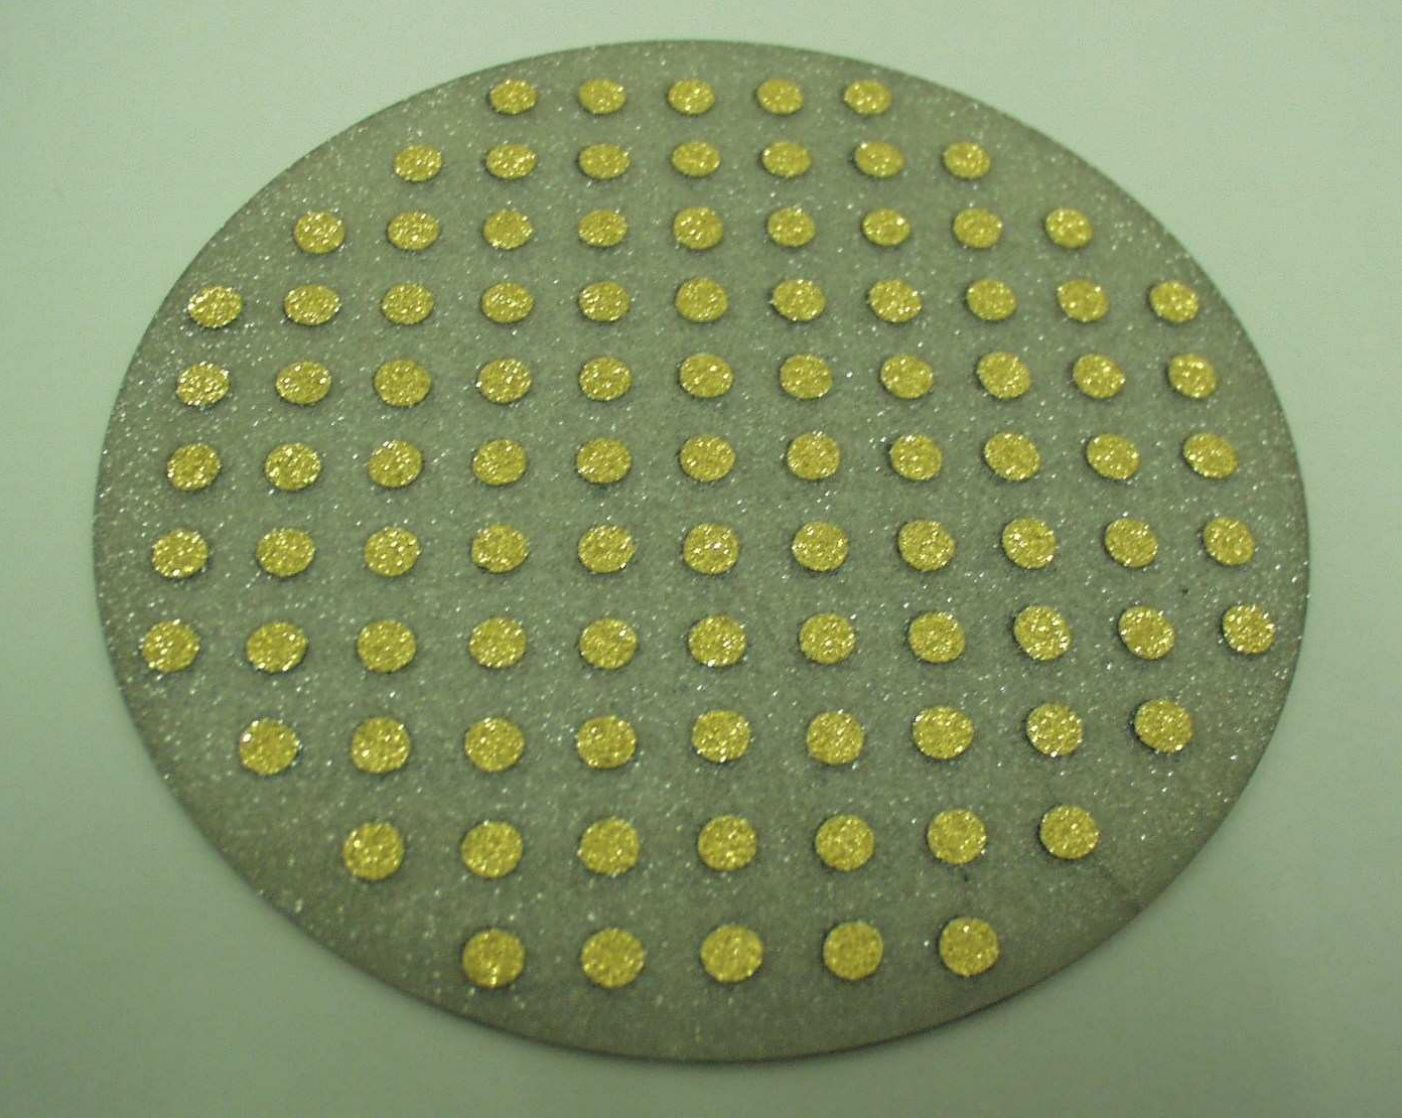
\includegraphics[width=0.7\textwidth]{04_charge_monitoring/pics/wafer}
\caption{A pCVD wafer. The golden dots on the surface are the electrodes that are applied during the qualification test. The wafer is measured across the surface to find the regions with the highest efficiency.}
\label{fig:wafer}
\end{figure}
\item[Silicon sensors] are standard $n^+ - in - n$ planar sensors with a 200~$\upmu$m thickness and were fabricated at CiS~\cite{CIS:00000}, a company from Erfurt, Germany. They are designed to have nearly a 100~\% efficiency when not irradiated. 
%Their bulk resistivity is between 2--5~k$\Omega$cm and they were diffusion oxygenated at 1150~\textdegree C for 24~hours to increase their radiation hardness. 
One side is segmented into pixels. Guard rings at the edges of the sensor provide a controlled drop in potential, reducing the possibility of shorts at maximum design bias voltages of the order of 1000~V.
\end{description}



\subsection{Front-end electronics}
The FE-I4 (front-end version four)~\cite{Albert:1477014} is an ASIC pixel chip designed specifically for the ATLAS pixel detector upgrade. It is built as a successor to the current pixel chip FE-I3, surpassing it in size of the active area (6$\times$ larger) as well as the number of channels/pixels (10$\times$ more). 336 such FE-I4 modules are used in the newly installed pixel layer called the Insertable B-Layer (IBL)~\cite{Huegging:1314083}. The DBM is also instrumented with these chips. The FE-I4's integrated circuit contains readout circuitry for 26880 pixels arranged in 80 columns on a 250~$\upmu$m pitch and 336 rows on a 50~$\upmu$m pitch. The size of the active area is therefore 20.0$\times$16.8~mm$^2$. This fine granularity allows for a high-precision particle tracking. The chip operates at 40~MHz with a 25~ns acquisition window, which corresponds to the spacing of the particle bunches in the LHC. It is hence able to correlate hits/tracks to their corresponding bunch. Furthermore, each pixel is capable of measuring the deposited charge of a detected particle by using the Time-over-Threshold (ToT) method. Finally, the FEI4 has been designed to withstand a radiation dose up to 300 MGy. This ensures a longterm stability in the radiation hard forward region of the ATLAS experiment.

\begin{figure}[!t]
\centering
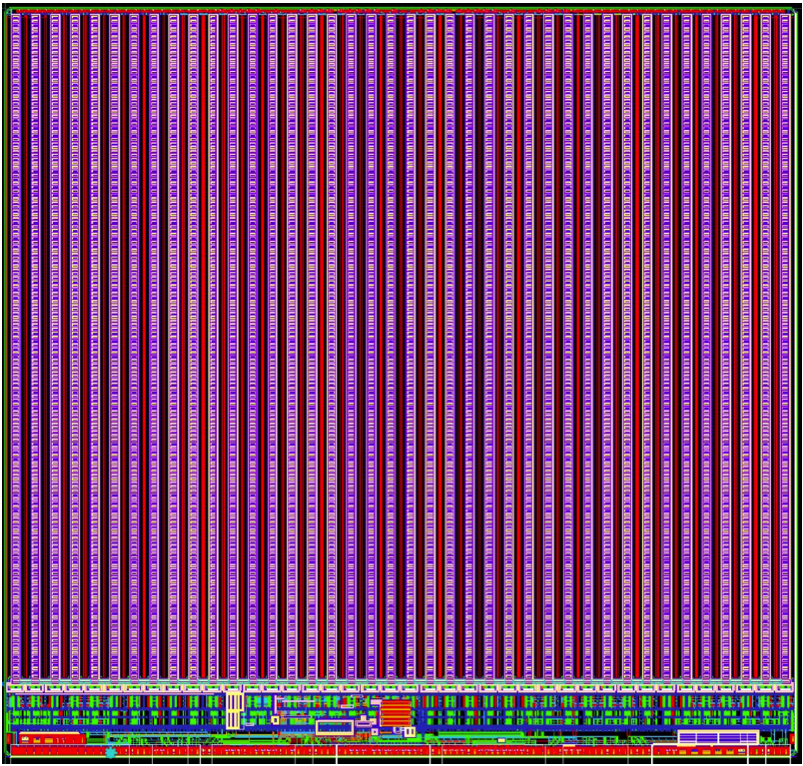
\includegraphics[width=0.6\textwidth]{04_charge_monitoring/pics/fei41}
\caption{FE-I4 layout, top-down view. The pink area are pixels grouped into columns, the green area below is the common logic and the red strip at the bottom are the wire bond pads.}
\label{fig:anapix}
\end{figure}

Each pixel is designed as a separate entity. Its electrical chain is shown in figure~\ref{fig:anapix}. The bump-bond pad -- the connection to the outside of the chip -- is the input of the electrical chain, connected to a free-running amplification stage with adjustable shaping using a 4-bit register at the feedback branch. The analog amplifier is designed to collect negative charge, therefore electrons. The output is routed through a discriminator with an adjustable threshold. This value in effect defines the level at which the circuit detects a hit. In addition, there is a counter of the clock cycles (25~ns sampling) during which the signal is above the discriminator threshold. The value of the counter is proportional to the collected charge. The logic gates at the end of the chain are used to enable/disable the pixel and to issue a so-called HitOr flag -- this signal is set whenever at least one of the pixels was hit and is used as a trigger for the readout. The output of the chain -- HitOut -- is routed into the logic of the chip where it is buffered and sent out to the readout system. The module receives all its commands from the system via a 40~MHz LVDS line. The commands are either settings for the pixel registers or triggers that start the data readout. The data are sent via an LVDS line at up to 320~Mbit/s, but by default at 160~Mbit/s, four times faster than the clock of the device. This allows the chip to clear out its buffers before new data are recorded, thus avoiding dead time and data pile-up. The FE-I4 has been successfully tested for trigger rates of up to 300~kHz, depending on the occupancy per trigger. 

\begin{figure}[!t]
\centering
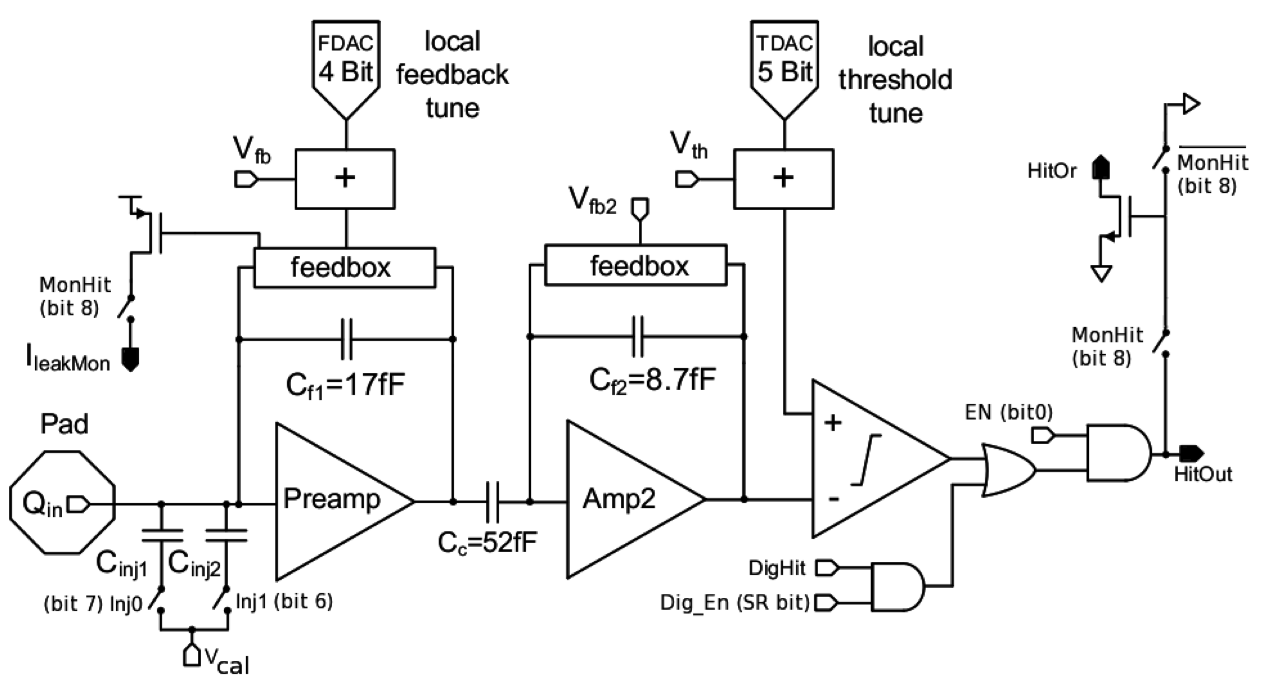
\includegraphics[width=0.7\textwidth]{04_charge_monitoring/pics/analogPix}
\caption{Schematic of an analog pixel. Courtesy of the FE-I4 collaboration.}
\label{fig:anapix}
\end{figure}

%describe threshold and IF tuning
The DBM uses pCVD diamond with $d_\mathrm{C}=500~\upmu$m thickness and silicon with $d_\mathrm{Si}=200~\upmu$m thickness as a sensor material. The resulting most probable value (MPV) of the deposited charge for a minimum ionising particle (MIP) is calculated with the formula $Q_\mathrm{S}=d \cdot E_\mathrm{e-h}$ and equals 18000~electrons and 17800~electrons, respectively, at a full charge collection efficiency. Unfortunately this is not the case with the pCVD material, whereby the expected charge collection efficiency is of the order of 50~\%  -- around 9000~e. This value further decreases with received irradiation dose. Therefore in order to detect the particles depositing energy on the far left side of the landau spectrum, the threshold has to be set to a significantly lower value. On the other hand, if the threshold set too low, it also detects the electronic noise and generates false hits. Typical noise amplitudes are in the range of 120--200~e. A safe threshold range is approximately five times above this value. The target for the DBM is to set the threshold to 800~e.

The analog amplifier is implemented in two stages to get a fast rise time at a low noise and a low power consumption. The output signal of the analog amplifier has a triangular shape with a fast rise time and a long decay.  The shape can be adjusted by tuning the amplifier feedback loop. Its length is proportional to the collected charge, but it needs to be calibrated first. This is done by means of two injection capacitors, $C_\mathrm{inj1}$ and $C_\mathrm{inj2}$, seen in figure~\ref{fig:anapix} with well defined capacitances. First, the charge $Q_\mathrm{cal}=V_\mathrm{cal}\cdot(C_\mathrm{inj1}+C_\mathrm{inj2})$ is injected into the analog chain. Then the length of the output pulse is measured and finally the feedback value is changed to either lengthen or shorten the pulse in order to get to the required duration $t_\mathrm{cal}$. The typical values are $Q_\mathrm{cal}=5000-16000~$e at the time $t_\mathrm{cal}=5-10~$ToT. The target values depend on the sensor, the type of a radioactive source and the application. Therefore the initial threshold $Th$ at 1~ToT and the calibrated value $Q_\mathrm{cal}$ at $t_\mathrm{cal}$~ToT give us a linear scale of collected charge with respect to time over threshold.
However, in practice this relation is nonlinear for lower thresholds, but since the goal of the measurements is to track the particles rather than to measure their deposited energy precisely, this is sufficient. 
 %The target values depend on the type of the sensor and the intended use of the device.
% It is capable of carrying out position-resolved measurements by performing high-precision particle tracking.
%Currently, the ATLAS pixel detector consists of three layers of silicon pixel sensors utilising the FE-I3 front-end ASIC pixel readout chips. In order to increase the impact parameter resolution of the detector, a fourth layer of sensors will be installed around the beam pipe. 


%---------------------------------------------------------------------------------------------------------------
\section{Module assembly}
\label{sec:modass}
%---------------------------------------------------------------------------------------------------------------
Parts for the detector arrived separately and were assembled into modules at CERN's DSF lab after being checked for production faults. The assembled modules underwent a series of quality control (QC) and burn-in tests to determine their quality, efficiency and long-term stability.

A DBM single-chip module consists of a hybrid pixel module, a flexible PCB and the supporting mechanics (a ceramic plate and an aluminium plate). The chip arrives already bump-bonded to the sensor, be it diamond or silicon. First it is glued to the ceramic plate on one side and to the PCB on the other using Araldite 2011 or Staystik 672/472. 
%The choice of glue was a topic of a lengthy discussion. 
Staystik is re-workable and has a very high thermal conductivity. The latter is important because the FE-I4 chips tend to heat up significantly and need a good heat sink. The problem is that it has a curing temperature of 160/170~\textdegree C. This temperature may cause some unwanted stress build-up between the FE-I4 and the diamond sensor due to different coefficients of thermal expansion, pulling them apart. This would disconnect the pixels, yielding large regions of the module insensitive to radiation. Araldite~2011 on the other hand can be cured at lower temperatures -- down to RT -- but it has a lower heat conductivity. In the end Araldite is used as a safer option. However, due to the longer curing, the entire assembly process using Araldite is extended to two working days. After curing, the module is wire-bonded and attached to the aluminium plate using screws made up of a radiation-resistant PEEK plastic. They have to be tightened with a great care, because their screw head is only 0.2--0.6~mm away from the sensor edge -- the sensor displacement tolerance during gluing is of the order of 0.5~mm. Finally, the module is put in an aluminium carrier which protects it from mechanical damage or electrostatic discharges. Figure~\ref{fig:completedmod} shows an assembled module.


\begin{figure}[!t]
\centering
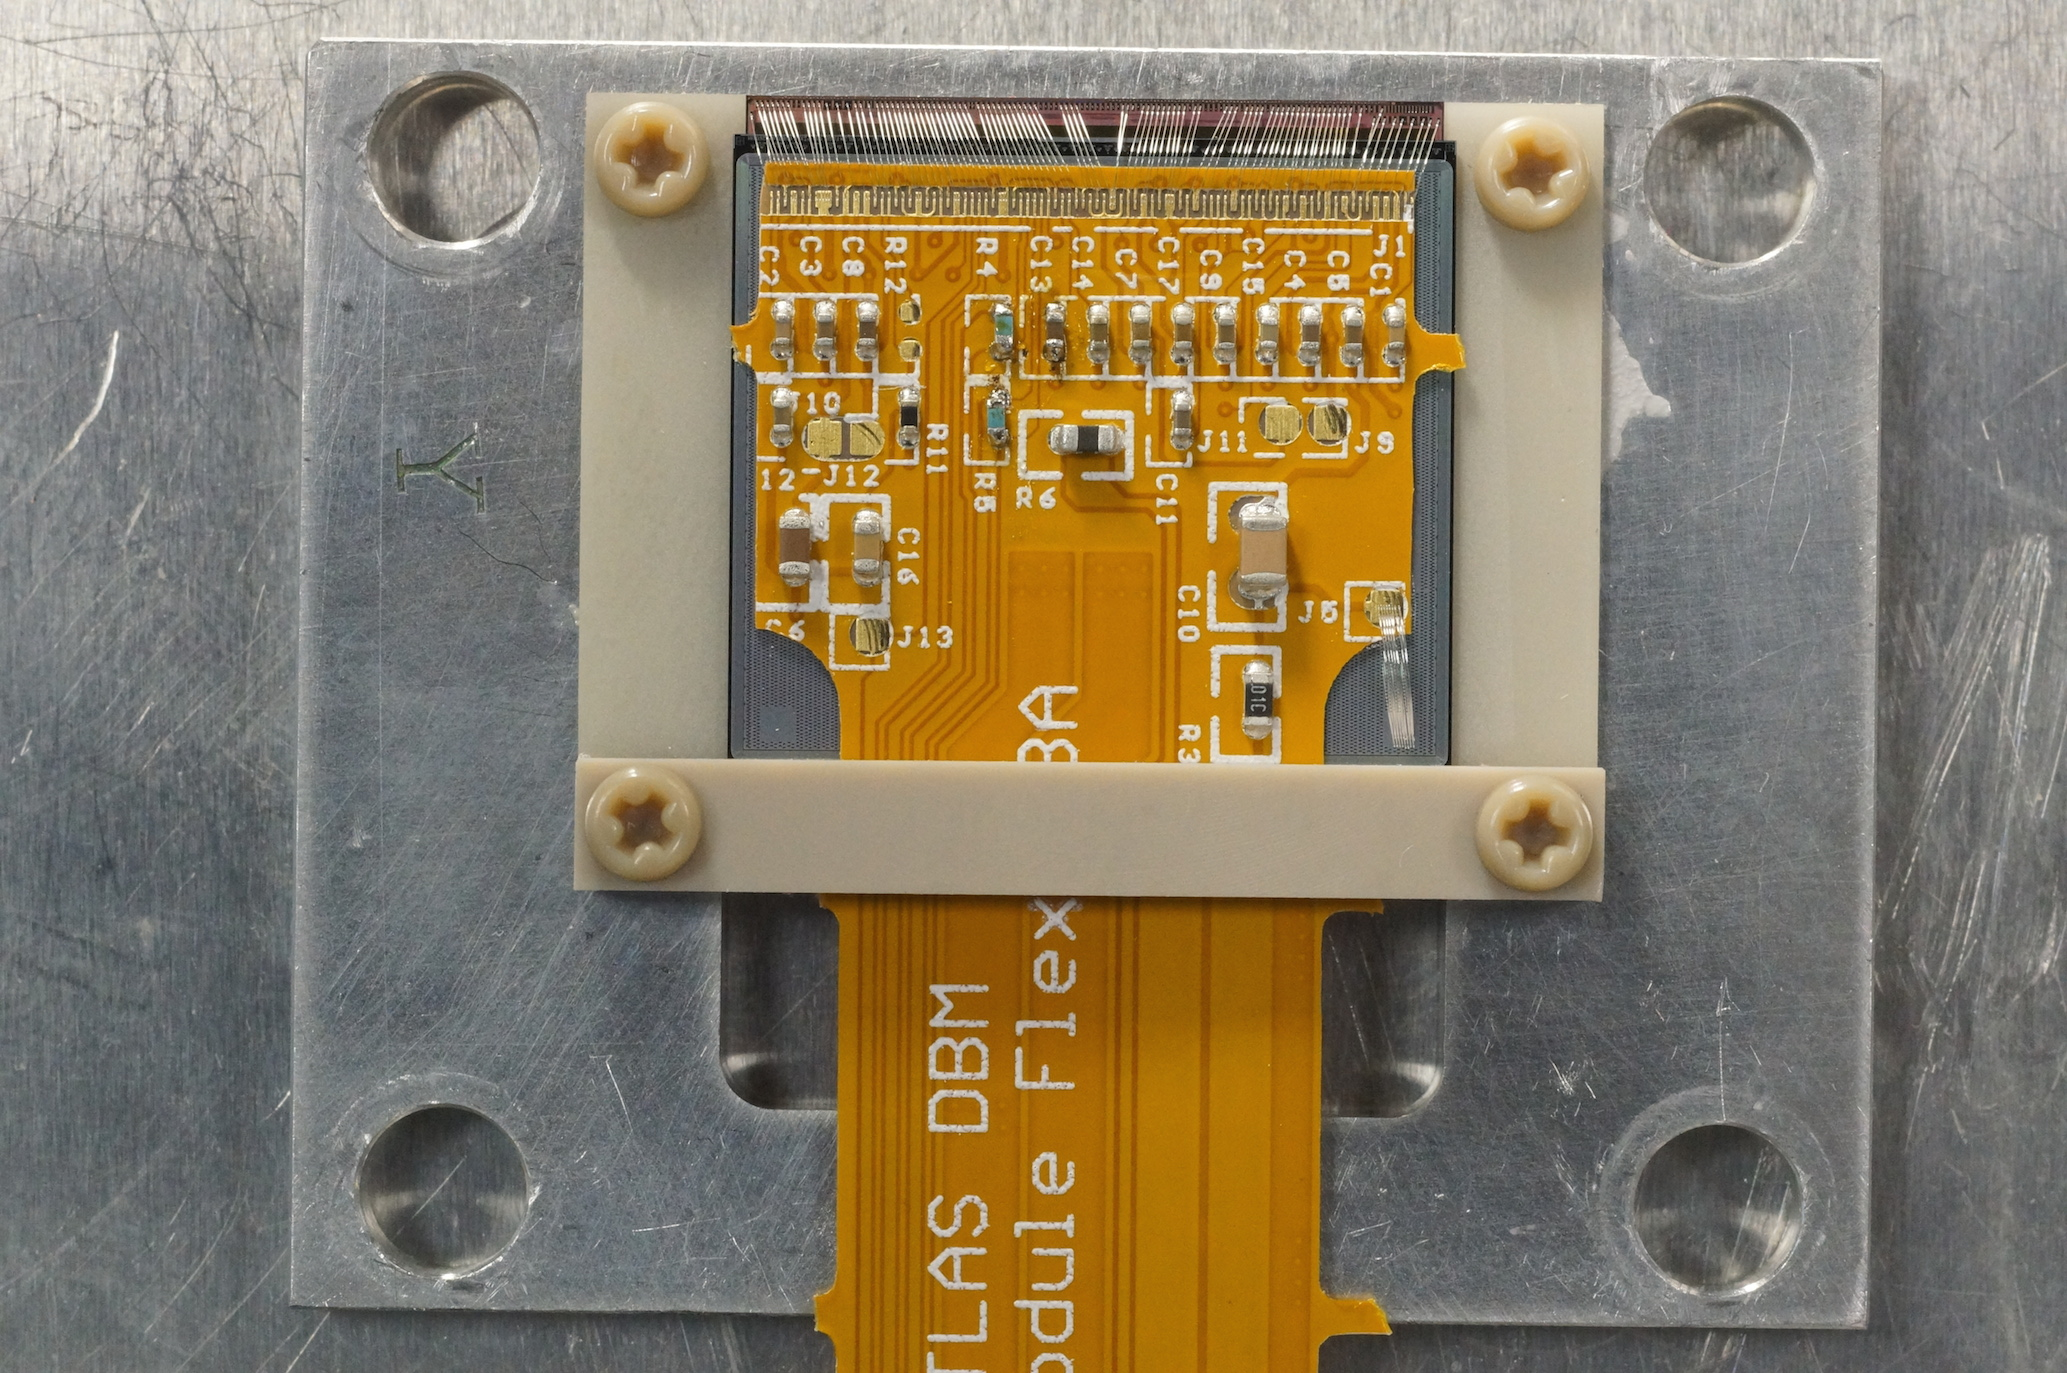
\includegraphics[width=0.7\textwidth]{04_charge_monitoring/pics/mod1}
\caption{DBM module, top-down view. Visible is the flexible PCB with signal and power connections, the silicon sensor and a part of the FE-I4. Wire bonds from the PCB to the FE-I4 and to the sensor are also visible.}
\label{fig:completedmod}
\end{figure}



%---------------------------------------------------------------------------------------------------------------
\section{Performance results}
\label{sec:perfresults}
%---------------------------------------------------------------------------------------------------------------
This section gives an overview of the performance results of the DBM modules achieved during the QC and the test beam campaign. The source tests were performed to check for disconnected regions in the sensors and to measure the diamond's efficiency. Only the modules with minimal disconnected regions and maximum efficiency were chosen for installation. 


\subsection{Source test results}
The modules are tested in the lab using an Reconfiguration Cluster Element readout system~\cite{Claus:2021543} and a moving stage with two degrees of freedom. They are placed onto the stage and connected to the readout system and the power supplies. After ensuring the low- and high voltage connectivity they are checked for the signal connectivity. If everything is operational, a series of automated tests is run. Each of these tests calibrates a certain value within a pixel, whether it is the signal threshold or the value for integrated charge. These are tuned in a way that the response to a predefined calibration signal is uniform for all pixels across the sensor. This procedure is referred to as \emph{tuning}. 

When the modules are tuned, they are tested using a $^{90}$Sr radioactive source. Two characteristics of each module are checked: 1) operation of all pixels and 2) sensor efficiency. 


\subsubsection{Pixel connectivity}
The first test is carried out to determine the number of disconnected pixels in the matrix.
This is an important step in the DBM QC procedure, because it turns out that a significant portion of the flip-chipped diamond sensors exhibited very poor connectivity. The disconnected regions on the faulty modules ranged anywhere from 0.5--80~\% of the overall active surface. In two cases the sensor was even completely detached from the chip. Therefore the pixel connectivity turns out to be the most important qualification factor in the QC procedure. Unfortunately the only way to check it at the moment is to fully assemble a module and test it using a radioactive source. If the module turns out to be of poor quality, it is disassembled and sent for rework. The turnover time of this operation is of the order of one month, which affected the DBM installation schedule significantly. In the end the modules with less then 3~\% disconnected pixels have been accepted.

\begin{figure}[!t]
%\centering
\begin{tabular}{cccc}
\subfloat[Occupancy scan for MSBM-34.]{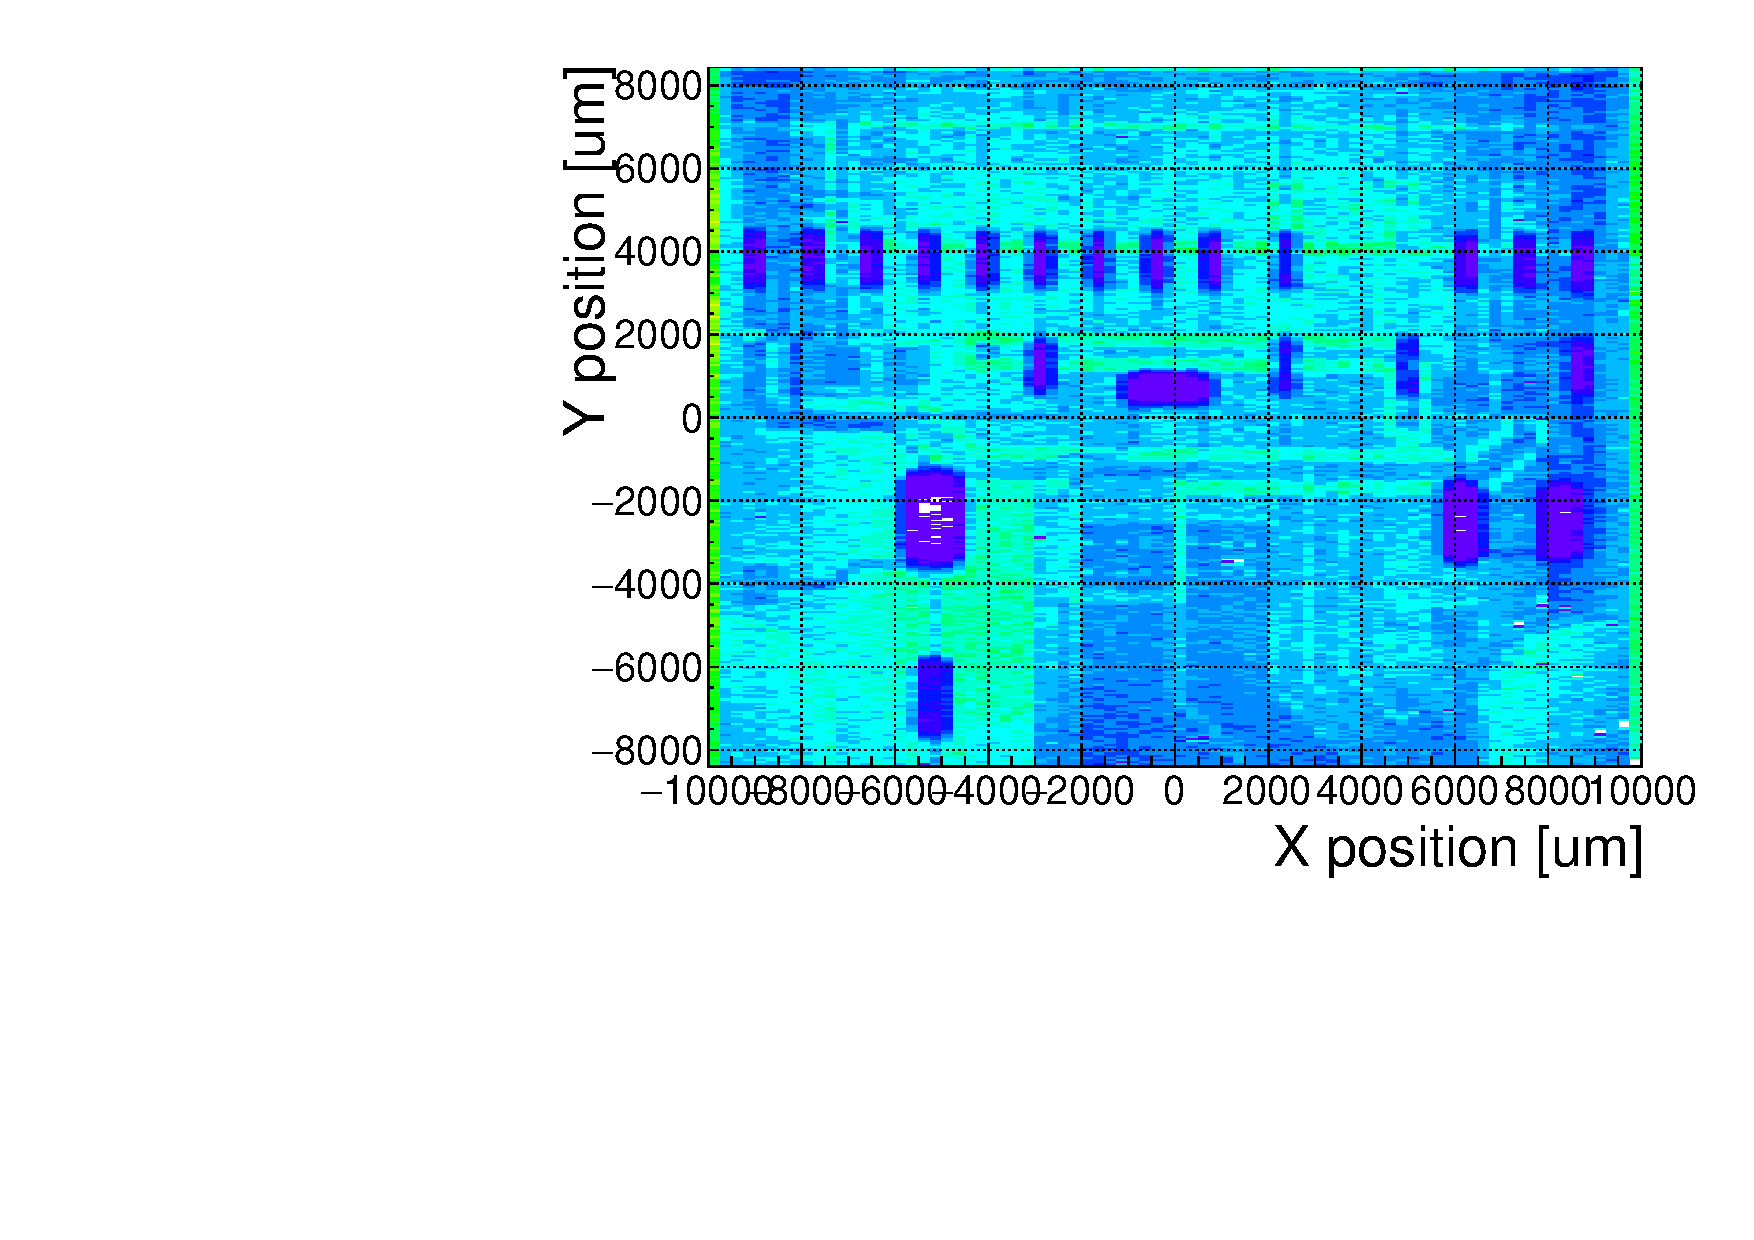
\includegraphics[width=0.45\textwidth]{../scripts/04_charge_monitoring/plots/MSBM-34-occ} \label{fig:MSBM-34-occ}} &
\subfloat[Occupancy scan for MDBM-23.]{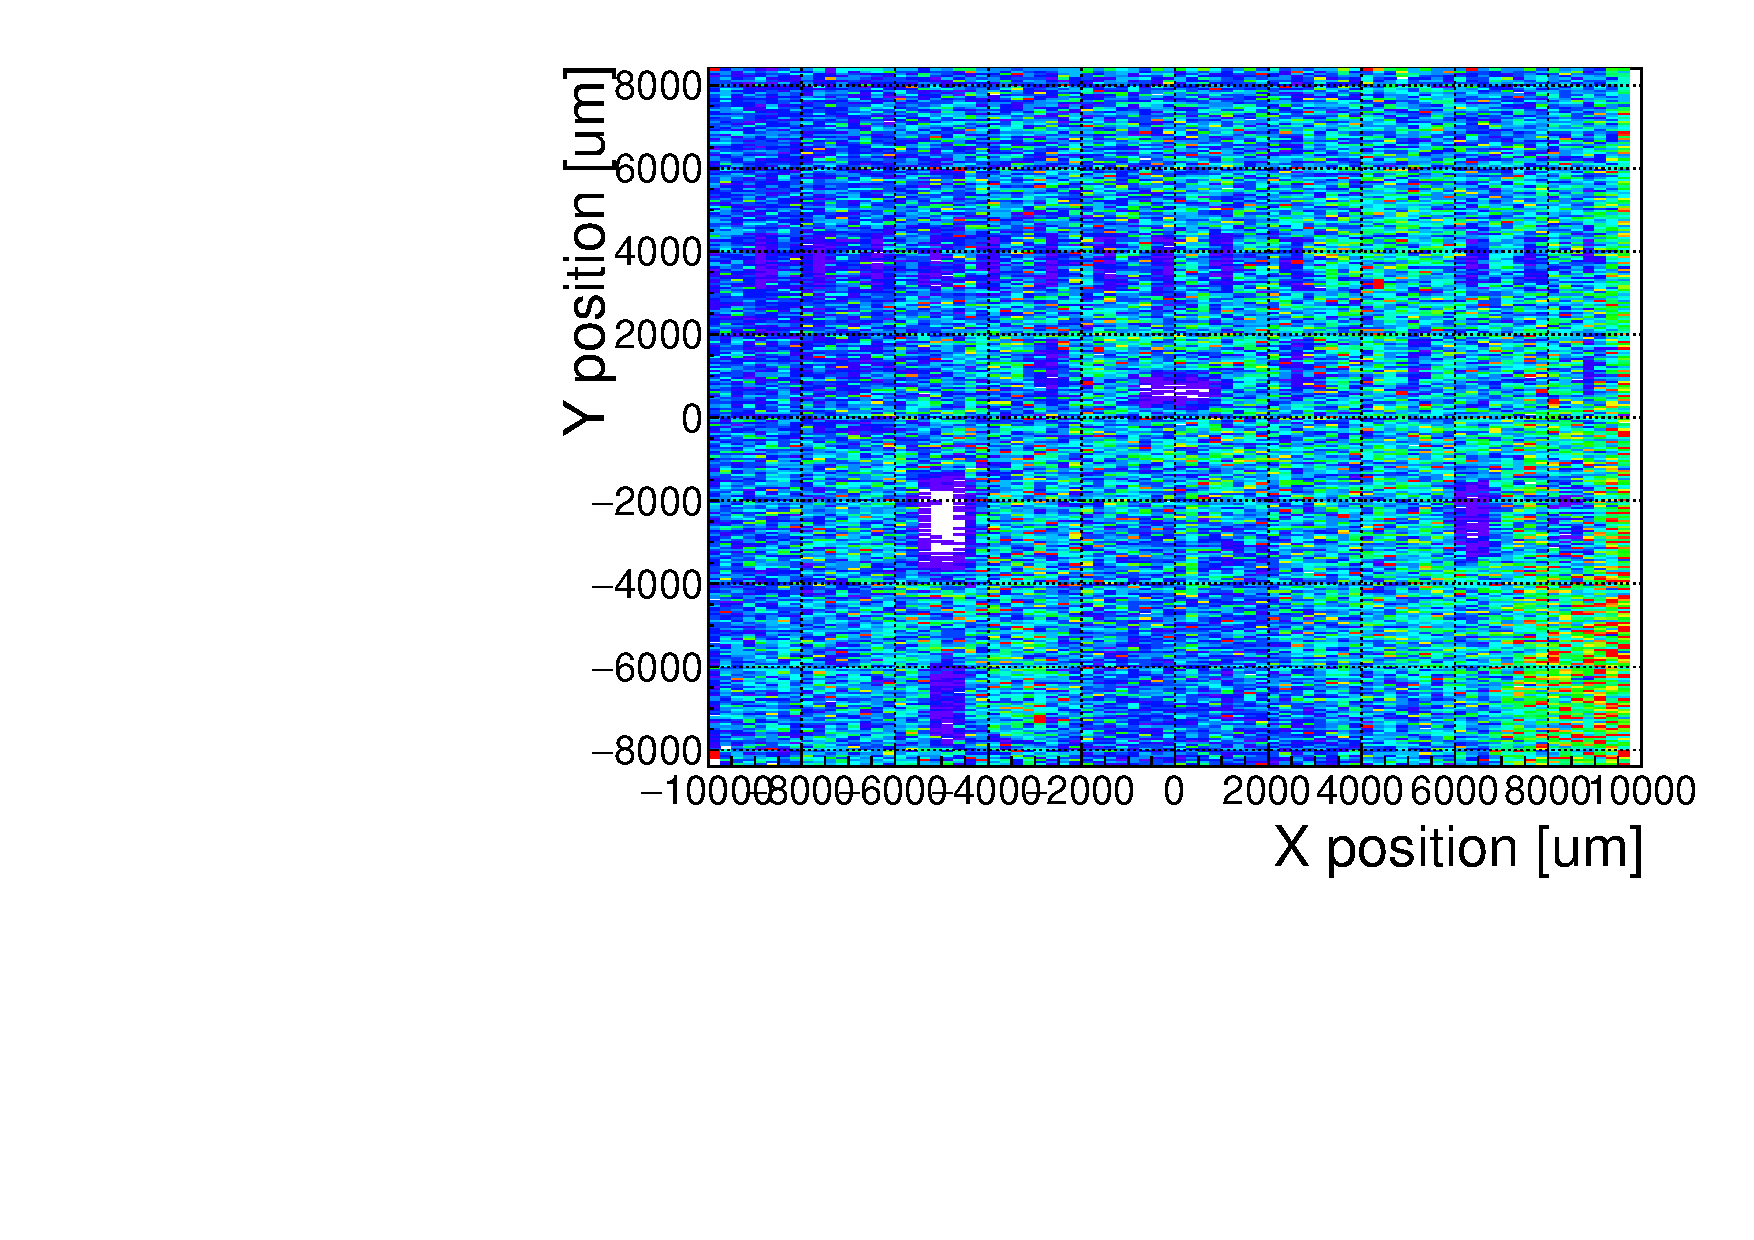
\includegraphics[width=0.45\textwidth]{../scripts/04_charge_monitoring/plots/MDBM-23-occ}  \label{fig:MDBM-23-occ}} \\
\end{tabular}
\caption{Occupancy scans for the silicon (left) and diamond sensor (right) to check for disconnected regions. Shadows of the electronic components are clearly visible because fewer electrons were able to traverse through such a higher amount of material.}
\end{figure}

The test for disconnected regions is carried out by moving the module under the source in X and Y direction so that the exposure over the entire plane is uniform. The resulting occupancy map reveals pixels that are not electrically coupled to the sensor via bump bonds. The occupancy scans are shown in figures~\ref{fig:MSBM-34-occ} and~\ref{fig:MDBM-23-occ}. The silicon module has a very uniform occupancy plot. So much so that the features of the overlaying flexible PCB can be observed. The rectangular shadows are the passive components whereas the lines are the traces in the PCB. Furthermore, a circular-shaped edge of the PCB can be seen on the bottom right side of the plot. These darker areas are such because fewer electrons can penetrate the material with a high density. In the case of the diamond, the features of the PCB can be observed as well, but are much less distinguishable as the plot is much more granulated -- less uniform. This high variance in the diamond's detection ability is due to the grain boundaries in the pCVD material which trap the drifting charges, rendering some regions significantly less efficient. 


\begin{figure}[!t]
\centering
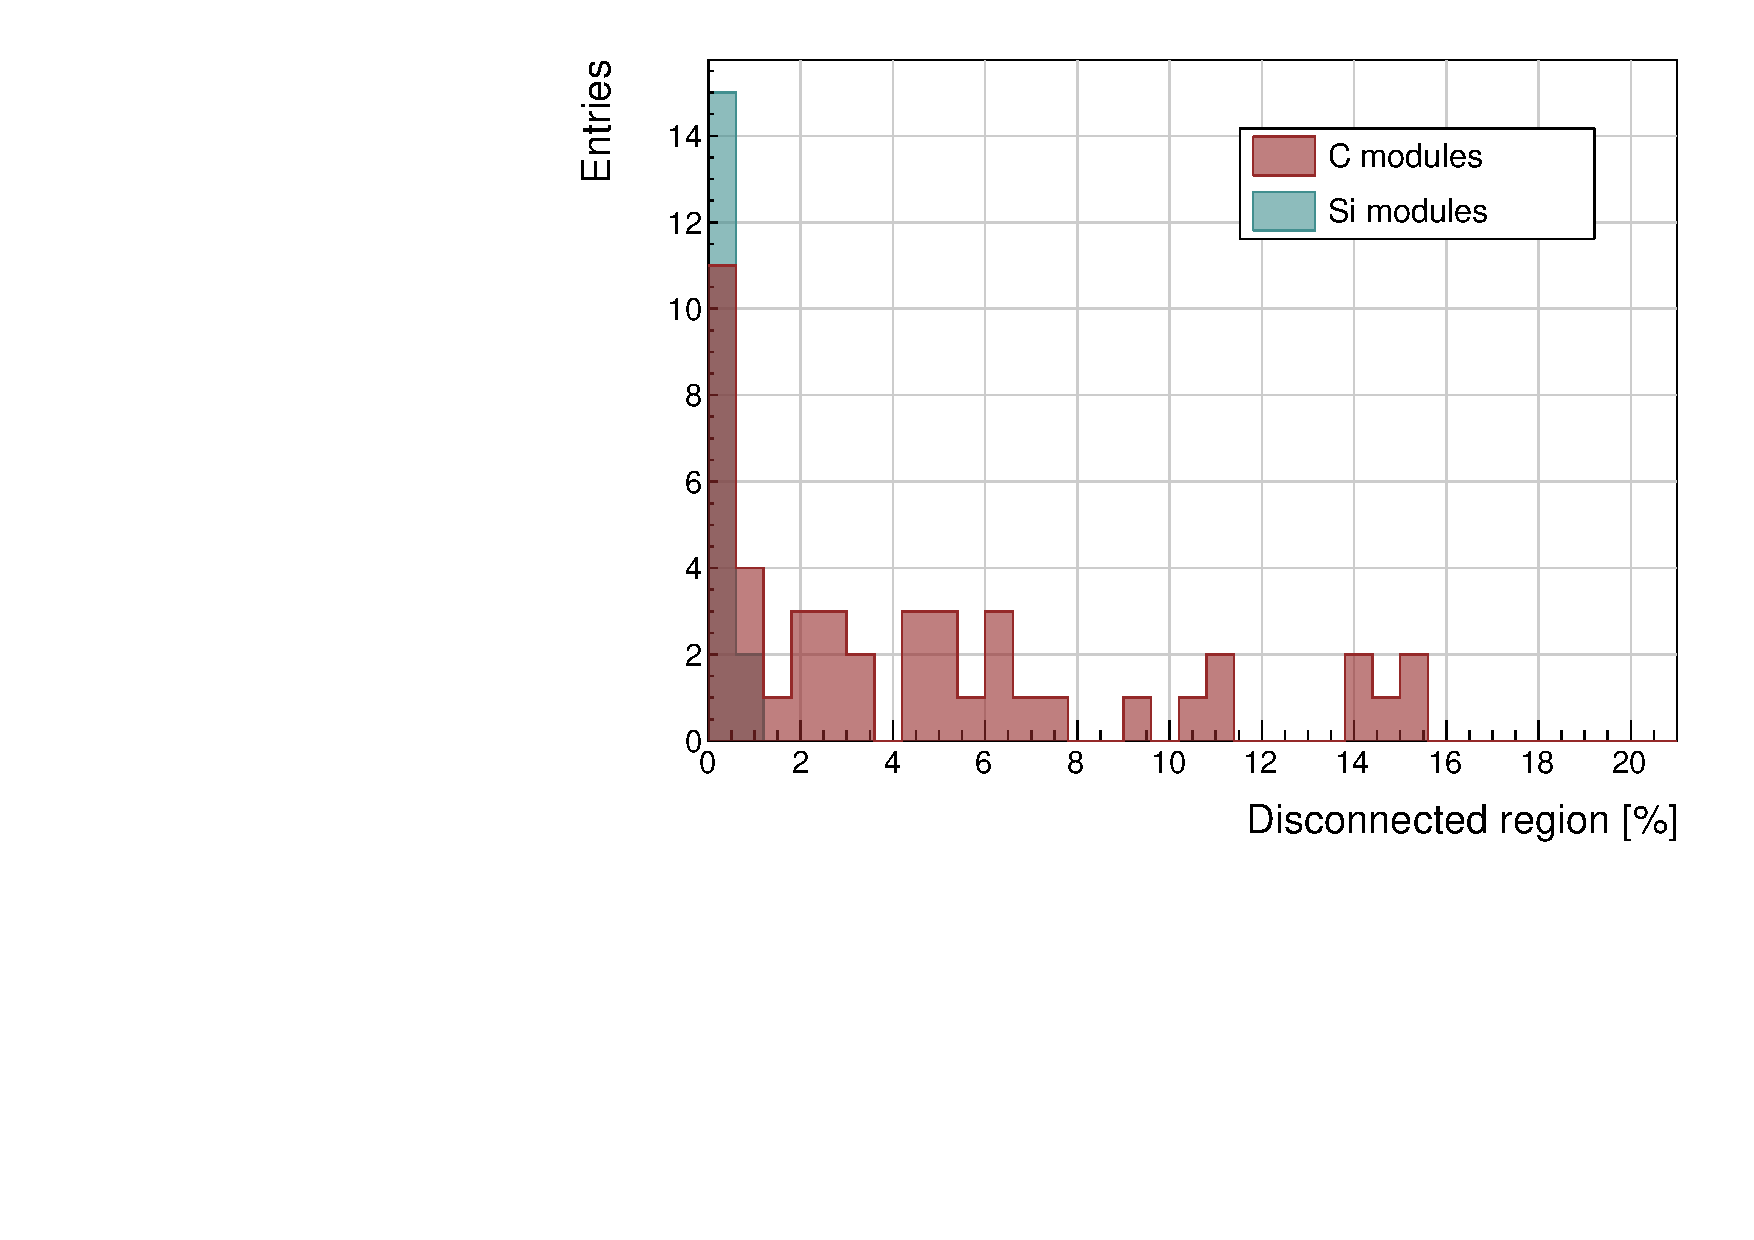
\includegraphics[width=0.7\textwidth]{../scripts/04_charge_monitoring/plots/disconnectedregion1} \caption{Disconnected regions for all modules derived from the occupancy scans.}
\label{fig:disconreg}
\end{figure}

Figure~\ref{fig:disconreg} shows the distribution of disconnected regions across all tested modules. Silicon modules were performing as expected, with a minimum number of disconnected pixels.




%--------------------------------------------------------------------------------------------------
\subsubsection{Pseudo-efficiency}
Only the modules that passed the pixel connectivity test undergo the second test stage in which the sensor's efficiency is estimated. A scintillator is placed underneath the module and is used as a trigger. A particle that crosses the DBM module and hits the scintillator, triggers the module readout. In the end, the number of triggers is compared to the number of hits/clusters recorded by the module. These are shown in figures~\ref{fig:MSBM-34-eff} and~\ref{fig:MDBM-23-eff}. 

\begin{figure}[!t]
%\centering
\begin{tabular}{cccc}
\subfloat[Pseudo-efficiency scan for MSBM-34.]{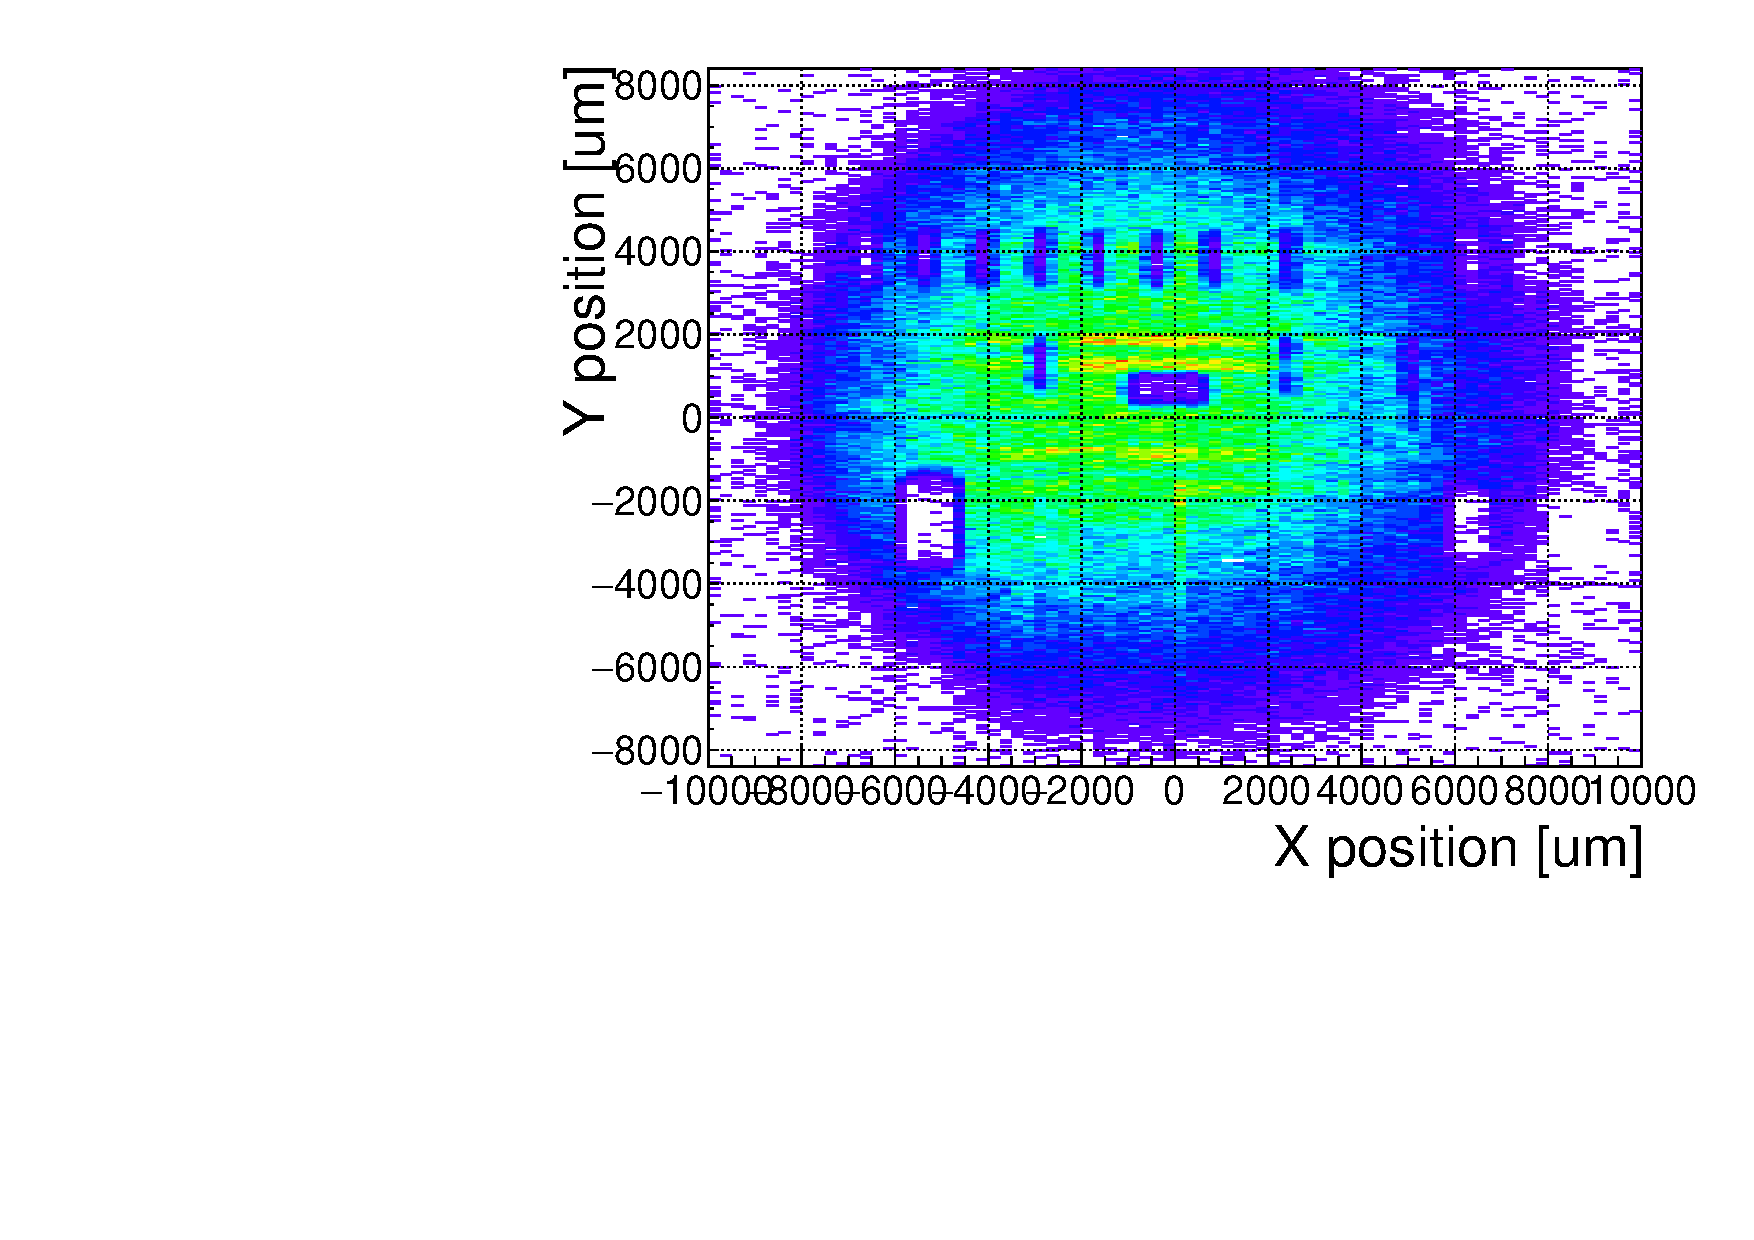
\includegraphics[width=0.45\textwidth]{../scripts/04_charge_monitoring/plots/MSBM-34-eff} \label{fig:MSBM-34-eff}} &
\subfloat[Pseudo-efficiency scan for MDBM-23.]{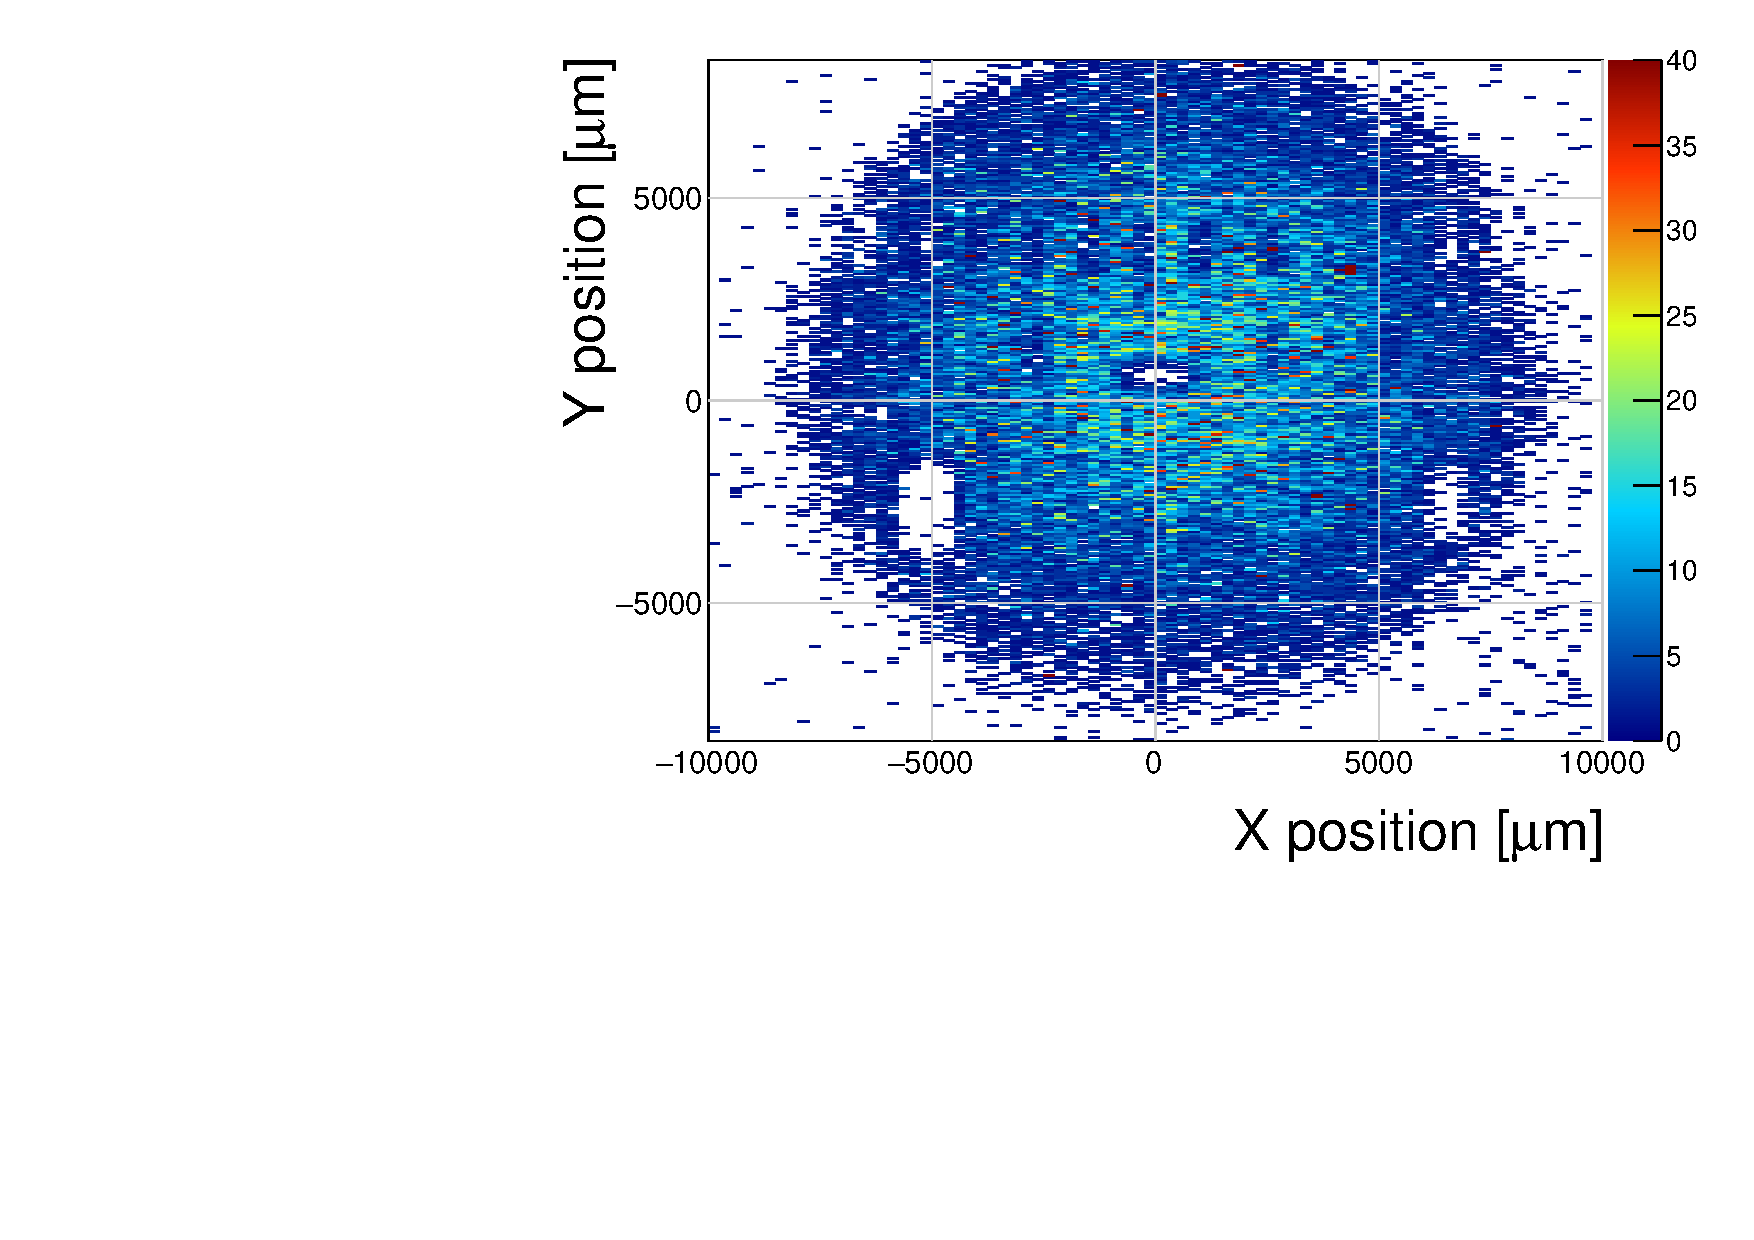
\includegraphics[width=0.45\textwidth]{../scripts/04_charge_monitoring/plots/MDBM-23-eff}  \label{fig:MDBM-23-eff}}
\end{tabular}
\caption{Pseudo-efficiency scans for the silicon (left) and diamond sensor (right) to estimate the efficiency of the sensors.}
\end{figure}

However, the resulting ratio is only an estimate of the sensor's detection efficiency. This is because the $\upbeta$ particles scatter around the setup and sometimes hit the scintillator from other directions without traversing the module, producing empty triggers. Therefore the real sensor efficiency can only be measured in a high energy particle beam and using a beam telescope as a reference detector to measure the particle trajectories. Nonetheless, this \emph{pseudo-efficiency} gives a rough estimate of the sensor's quality.

\begin{figure}[!t]
\centering
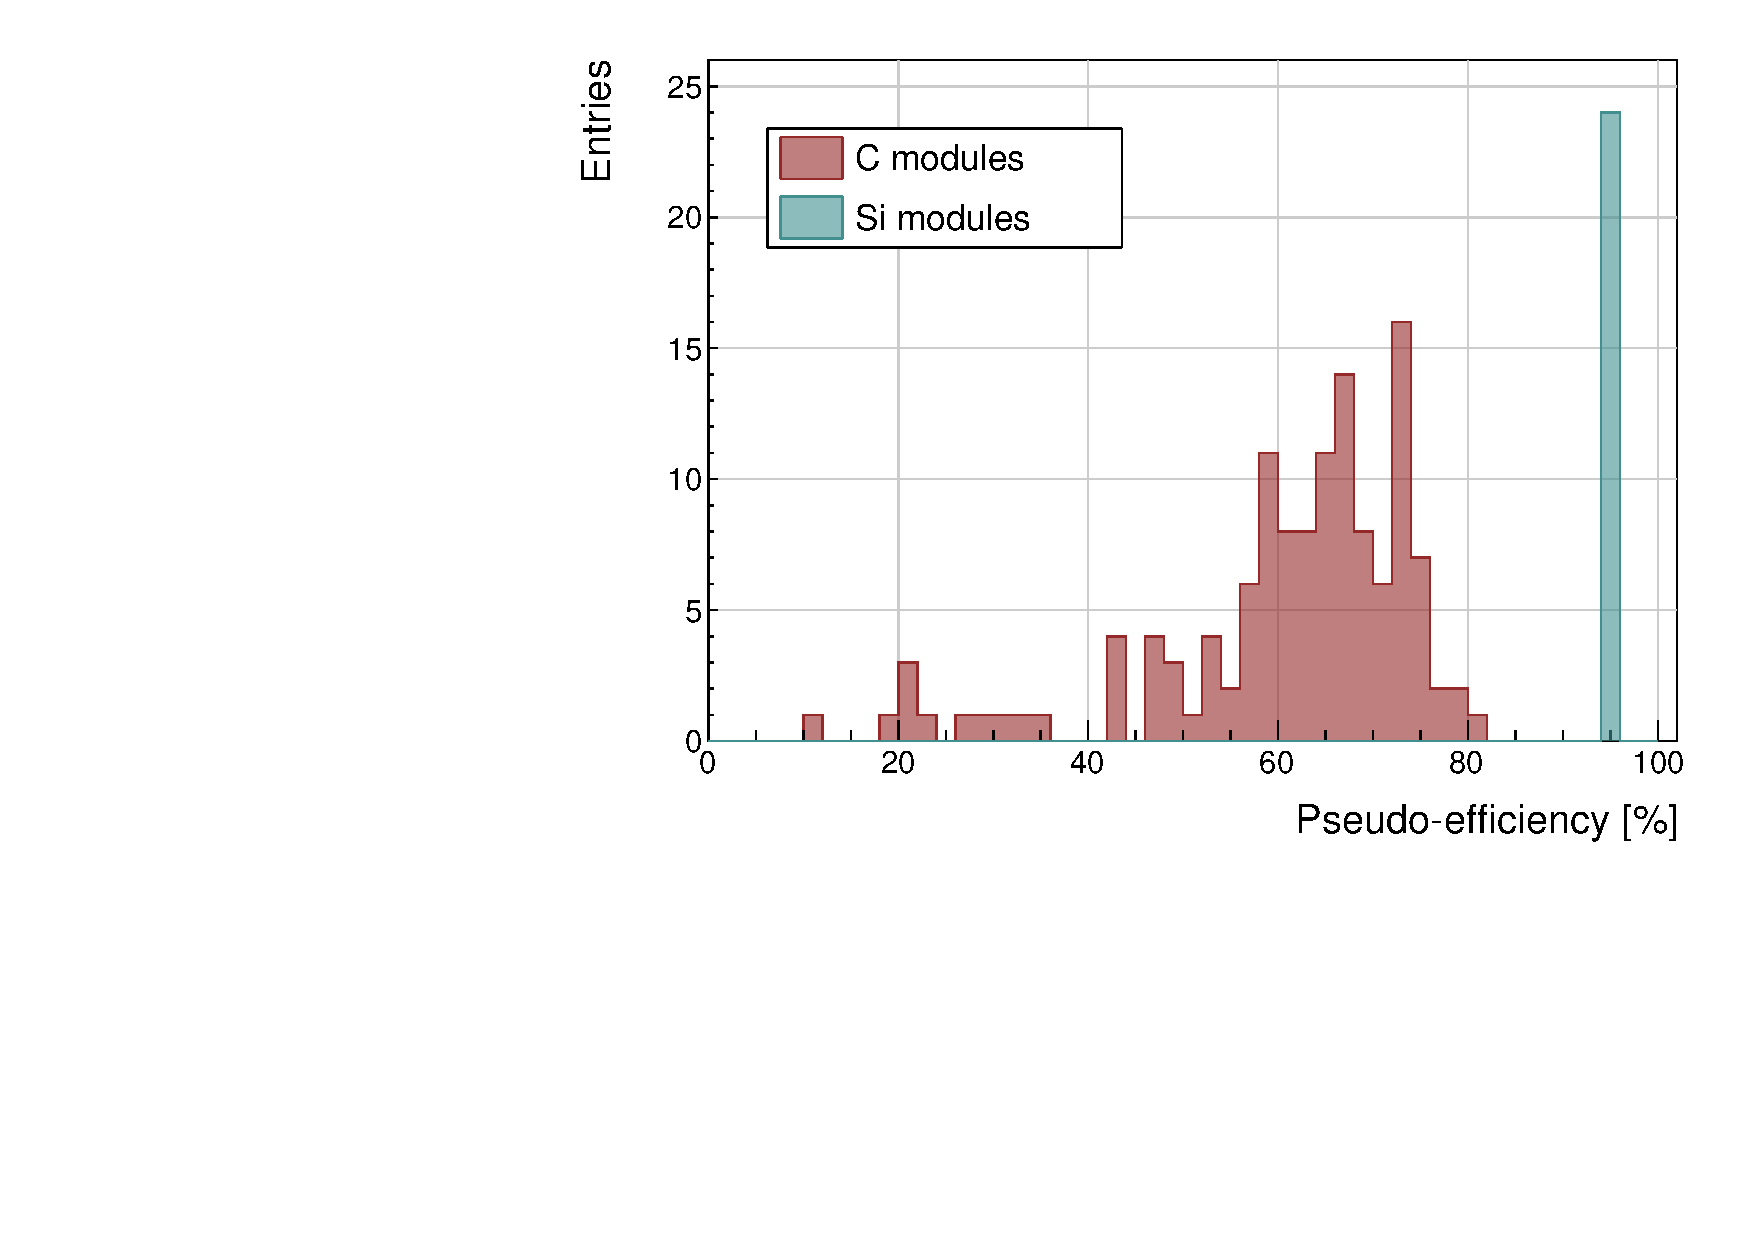
\includegraphics[width=0.7\textwidth]{../scripts/04_charge_monitoring/plots/pseudoefficiency1} 
\caption{Pseudo-efficiencies for all modules at various threshold and voltage settings.}
\label{fig:pseudoeff}
\end{figure}

Figure~\ref{fig:pseudoeff} shows the distribution of pseudo-efficiencies for all modules that went through the QC. The majority of the silicon modules yield the pseudo-efficiency of (94.3$\pm$0.2)~\%. Silicon sensors being 99.99~\% efficient, this value is underestimated by about 5~\%. The measured pseudo-efficiency of the diamond modules is $(65\pm7)$~\%, with outliers down to 10~\%. The value depends on the diamond quality, the set threshold and the applied bias voltage. The latter two settings are varied to check the behaviour of the modules under various conditions. 

%--------------------------------------------------------------------------------------------------
\subsection{Erratic current}
A very important parameter for qualifying a module is the erratic current~\cite{Mueller:1175553} in the sensor. This term describes the leakage current in a pCVD diamond that becomes unstable. It can develop gradually or can be triggered with a $\upbeta$ source. Spikes appear in the otherwise stable leakage current. They can be up to three orders of magnitude higher than the base current. Sometimes the current also suddenly increases for a few orders of magnitude and stays at that level (e.g. from the initial 1~nA to 3~$\upmu$A). An example of such behaviour is shown in figure~\ref{fig:erratic1}. 

The amplitude differs in magnitude from sensor to sensor. This effect is still not fully explained, but the hypothesis is that the charges find a conductive channel along the grain boundaries, causing discharges. These discharges are picked up by the pixel amplifiers in the FE-I4. A single discharge can trigger a group of up to $\sim$500 pixels, resulting in a \emph{blob} on the detector occupancy map. Sometimes the conductive channel stays in a conductive state, making one or more pixels always to fire. These pixels saturate the bandwidth of the readout channel, so they have to be masked out during measurements. 

\begin{figure}[!t]
\centering
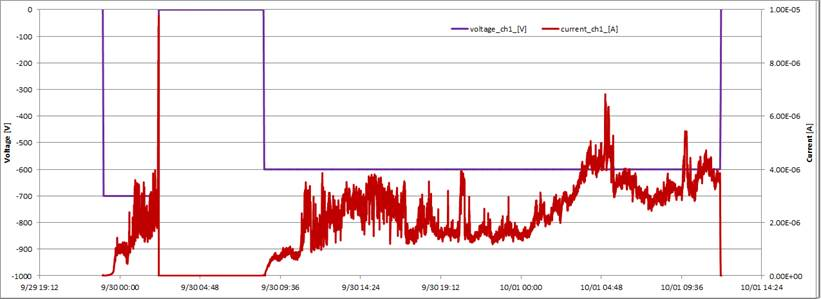
\includegraphics[width=0.7\textwidth]{04_charge_monitoring/pics/erratic1} 
\caption{Erratic current in a DBM diamond module.}
\label{fig:erratic1}
\end{figure}

%--------------------------------------------------------------------------------------------------
\subsection{Test beam results}
The first two assembled prototype DBM modules, MDBM-01 and MDBM-03, were tested at DESY, Hamburg, in a test beam facility. The aim of the measurements was to measure their efficiency, the spatial distribution of the efficiency and the effect of the beam on the disconnected regions. A silicon module MSBM-02 was measured to crosscheck the measurements. Since the silicon module is almost 100~\% efficient, it was used as an ``anchor'' -- the efficiency of the diamond module was measured relative to that of the silicon module. Two beam telescopes were used as reference systems: Kartel telescope~\cite{McGoldrick:1982209} built by JSI institute from Ljubljana, and EUDET Aconite~\cite{ACONI:00000}. Both are instrumented with six Mimosa26 pixel planes and capable of tracking particles with a 2~$\upmu$m pointing resolution.

The test beam prototypes did not meet the acceptance criteria for production DBM modules in the following areas: first, the stated CCDs were slightly below 200~$\upmu$m, which would be the DBM minimum. Secondly, the applied bias voltages ranged from 1--2~V/$\upmu$m. In addition, the threshold cut could only be set to 1500~electrons, which is higher than the DBM minimum (1000~e). Nonetheless, the resulting module efficiencies were still in the range between 70--85~\%.

To analyse the test beam data, Judith software framework~\cite{McGoldrick:1982209} was used. Judith is capable of synchronising data streams from several detector systems only connected via a trigger system, reconstructing tracks and calculating efficiency for the DUTs. It was also used to reconstruct and analyse the acquired Kartel test beam data together with the silicon and diamond module as DUTs. A sample of the analysed data is shown in figures~\ref{fig:beammap} and~\ref{fig:beamdist}. 


\begin{figure}[!t]
%\centering
\begin{tabular}{cccc}
\subfloat[This figure shows an efficiency map of ad DBM pVCD diamond module. Each bin corresponds to a single pixel. The triggering scintillator of the Kartel telescope is smaller than the DUT. Hence, the recorded hits can only be seen in the top half of the sensor. ]{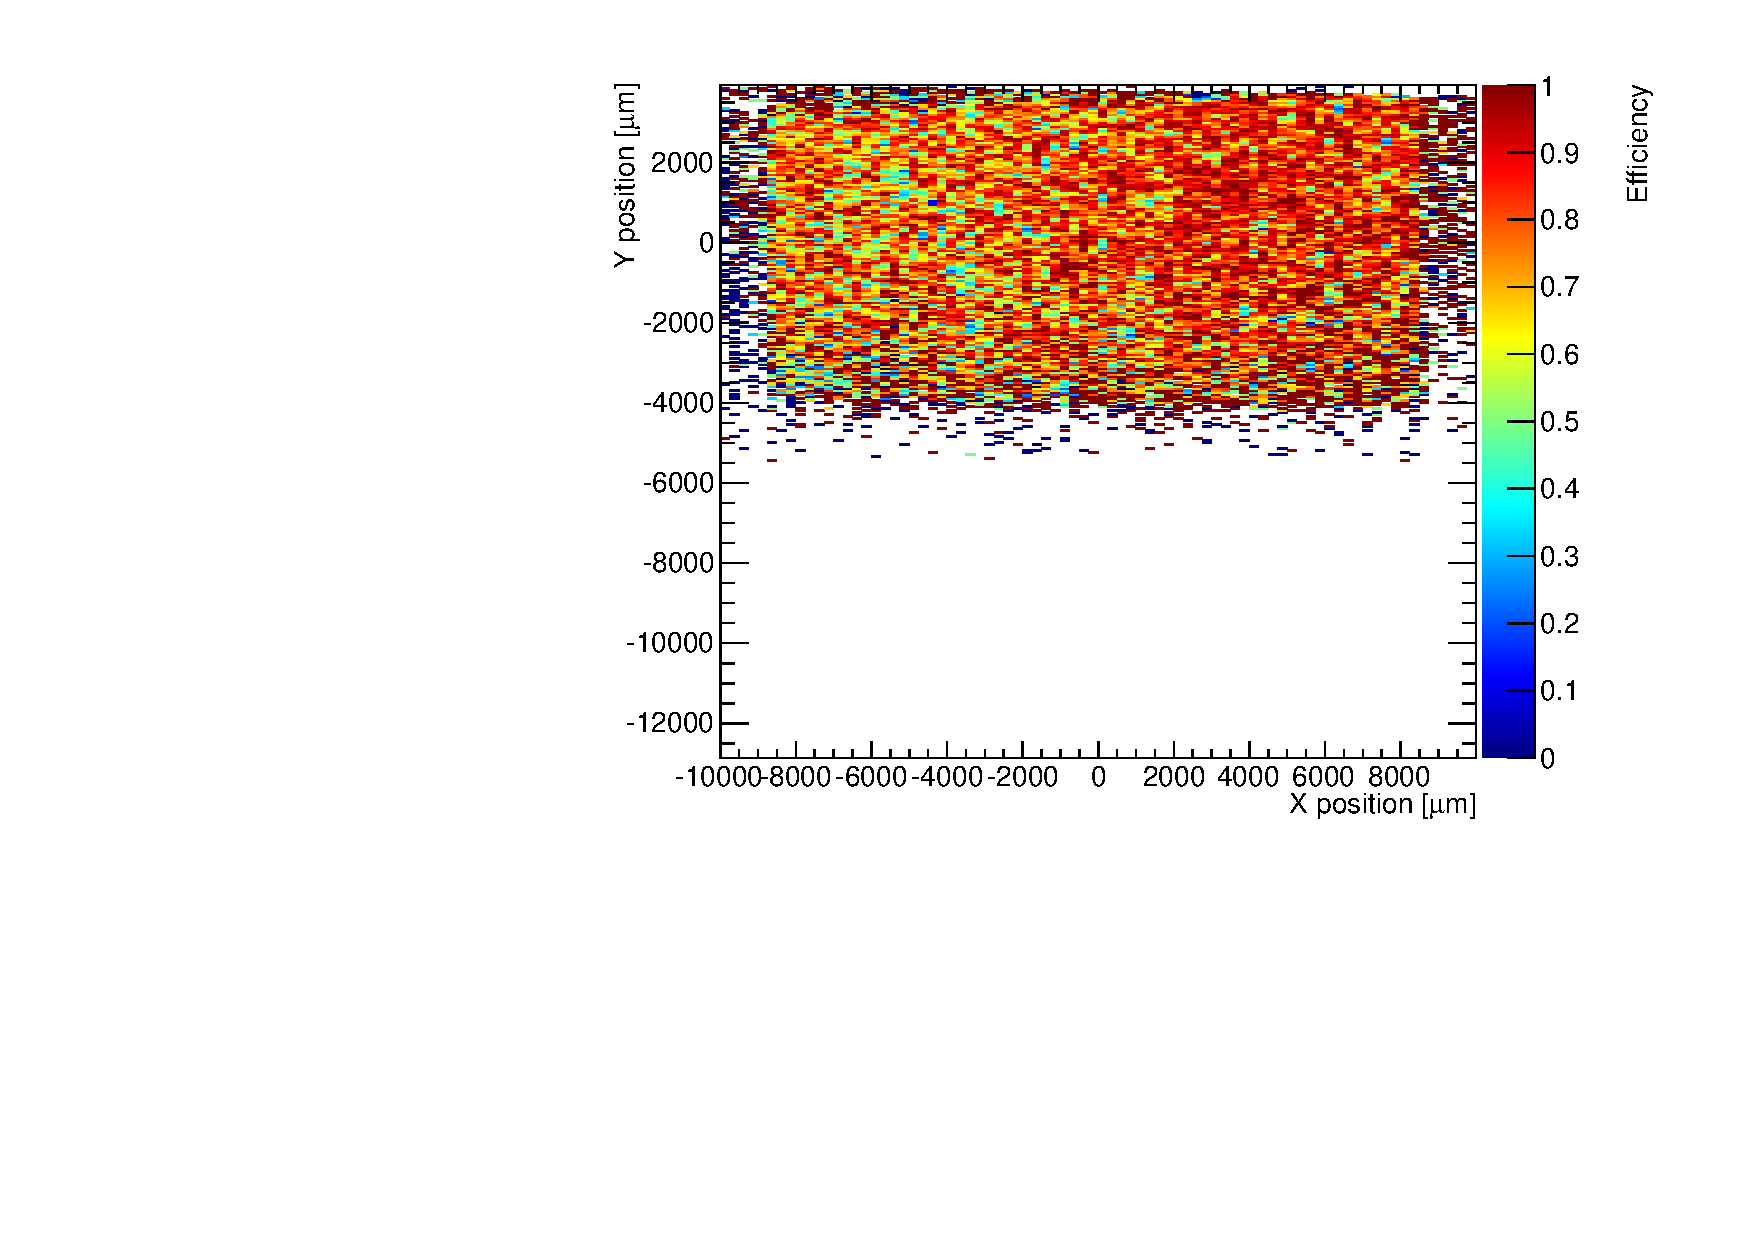
\includegraphics[width=0.45\textwidth]{../scripts/04_charge_monitoring/plots/map} \label{fig:beammap}} &
\subfloat[A pixel efficiency distribution from the run in figure (a).]{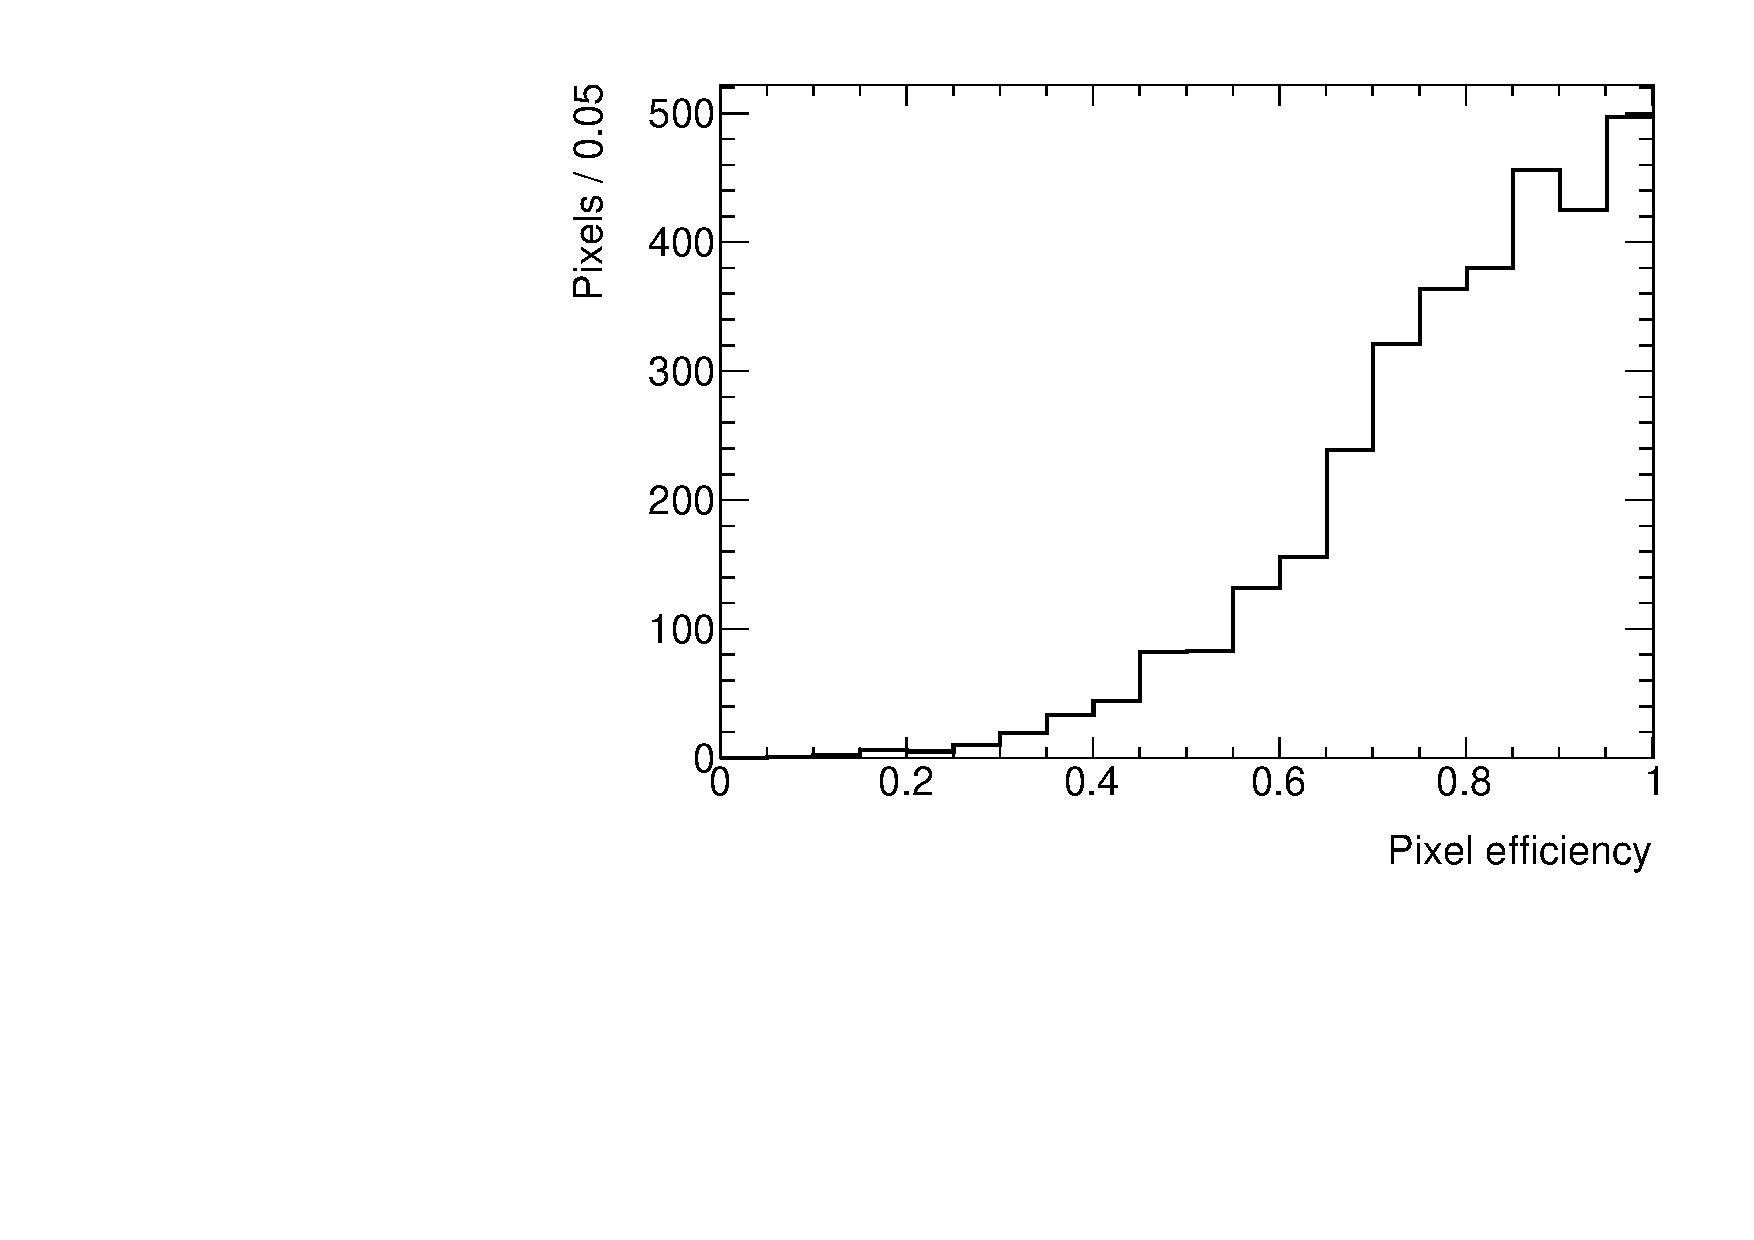
\includegraphics[width=0.45\textwidth]{../scripts/04_charge_monitoring/plots/distribution}  \label{fig:beamdist}}
\end{tabular}
\caption{An efficiency study of a prototype DBM diamond module in a test beam. The statistics are low ($\sim$~10~hits/pixel) as the data were collected during a short run. }
\end{figure}



%--------------------------------------------------------------------------------------------------
\subsection{Summary of the QC}
All in all, 79 modules went through the QC procedure -- 43 diamond modules and 36 silicon modules, 12 of the latter only for testing purposes. Figure~\ref{fig:production} shows their production with time. 18 diamond modules and 6 silicon modules were in the end chosen to be integrated into DBM telescopes and installed into ATLAS.


\begin{figure}[!t]
\centering
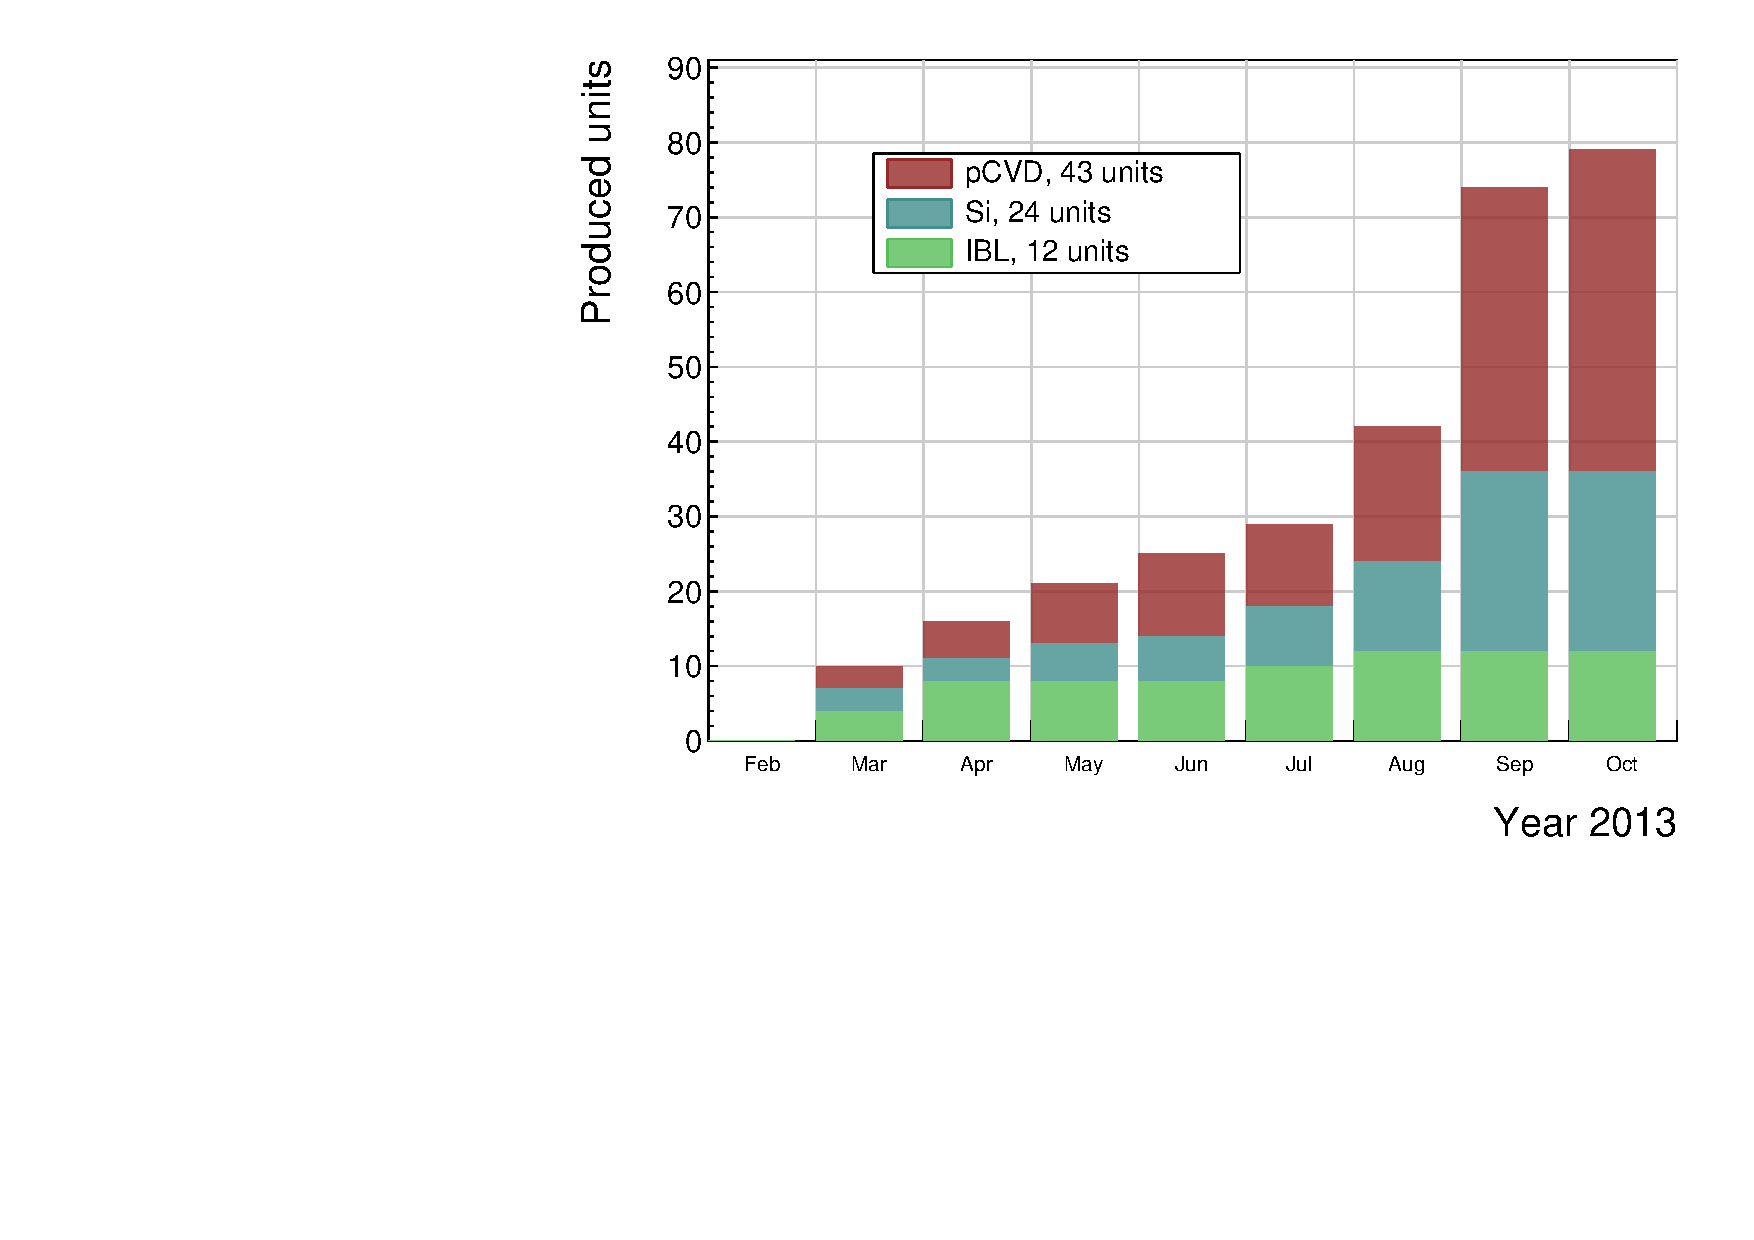
\includegraphics[width=0.7\textwidth]{../scripts/04_charge_monitoring/plots/production1}
\caption{Module production with time.}
\label{fig:production}
\end{figure}



















%---------------------------------------------------------------------------------------------------------------
\section{Installation and commissioning}
\label{sec:install}
%---------------------------------------------------------------------------------------------------------------

The DBM modules that passed the QC tests were assembled into telescopes -- sets of three modules one behind the other with a spacing of 50~mm. Of the 18 diamond and 6 silicon modules, 6 diamond and 2 silicon telescopes were built. A special care was taken when choosing the sets of three diamonds. The modules with a similar pseudo-efficiency, leakage current, maximum stable high voltage and shape of disconnected regions were grouped together. After assembly into telescopes, the modules were tested for their connectivity. Then the high voltage was applied and the leakage current was observed. This was an important point to check because all three modules shared the same high voltage channel. Any instabilities on one of the modules would cause problems on the other two. This would for instance happen if one of the modules had a much lower breakdown voltage.

Due to time constraints, the telescopes were not built at the same time but instead the production was pipelined. As soon as two telescopes were ready, they were transported to Point~1 -- the site where parts of the ATLAS detector were being put together. There they were prepared for installation onto the pixel detector structure that had been extracted from ATLAS due to pixel detector commissioning. The commissioning was nearing completion, so the technicians were preparing the detector for re-insertion. The cylindrical structure was being enclosed by four new service quarter-panels (nSQPs). This meant that with with every day the access to the place of installation of the DBM was more difficult. The first two telescopes were still put into place when only one nSQP was in place. This allowed the installation process to be carried out from both sides. This proved to be helpful, because the process was lengthy and had to be done with great precision. It involved tightening several screws on both sides of the telescopes, adding thermal paste on the aluminium joints and removing the protective covers, revealing the fragile wire bonds. At the same time the surrounding electronics and cables had to be left untouched. The lessons learnt with the first part of the installation were helpful when installing the other telescopes. The last two were fitted onto the structure when three nSQPs were already in place, leaving only a narrow opening for access. The entire procedure was carried out blind. After every installation, the telescopes were tested again. First, the low voltage connectivity was checked and a set of tests was run on the FE-I4 front-end chips. An eye diagram was made to estimate the quality of the signal transmission. Then a $^{90}$Sr source was used to perform a source test on three modules at the same time. Leakage current was observed during the source test. The final test included running four telescopes (all on one side) at a time. All the tests were successful and the DBM was signed off.

\subsection{Positioning in ATLAS}
The DBM is placed in the forward region of the ATLAS detector very close to the beam pipe, as shown in figure~\ref{fig:dbminatlas}. Eight DBM telescopes reside approximately 1~m away from the collision region, four on each side. They are tilted with respect to the beam pipe for 10\textdegree. This is due to a specific phenomenon connected to erratic (dark) currents in diamond. Studies have shown~\cite{Mueller:1175553} that the erratic leakage currents that gradually develop in diamond can be suppressed under certain conditions. 
\begin{figure}[!t]
\centering
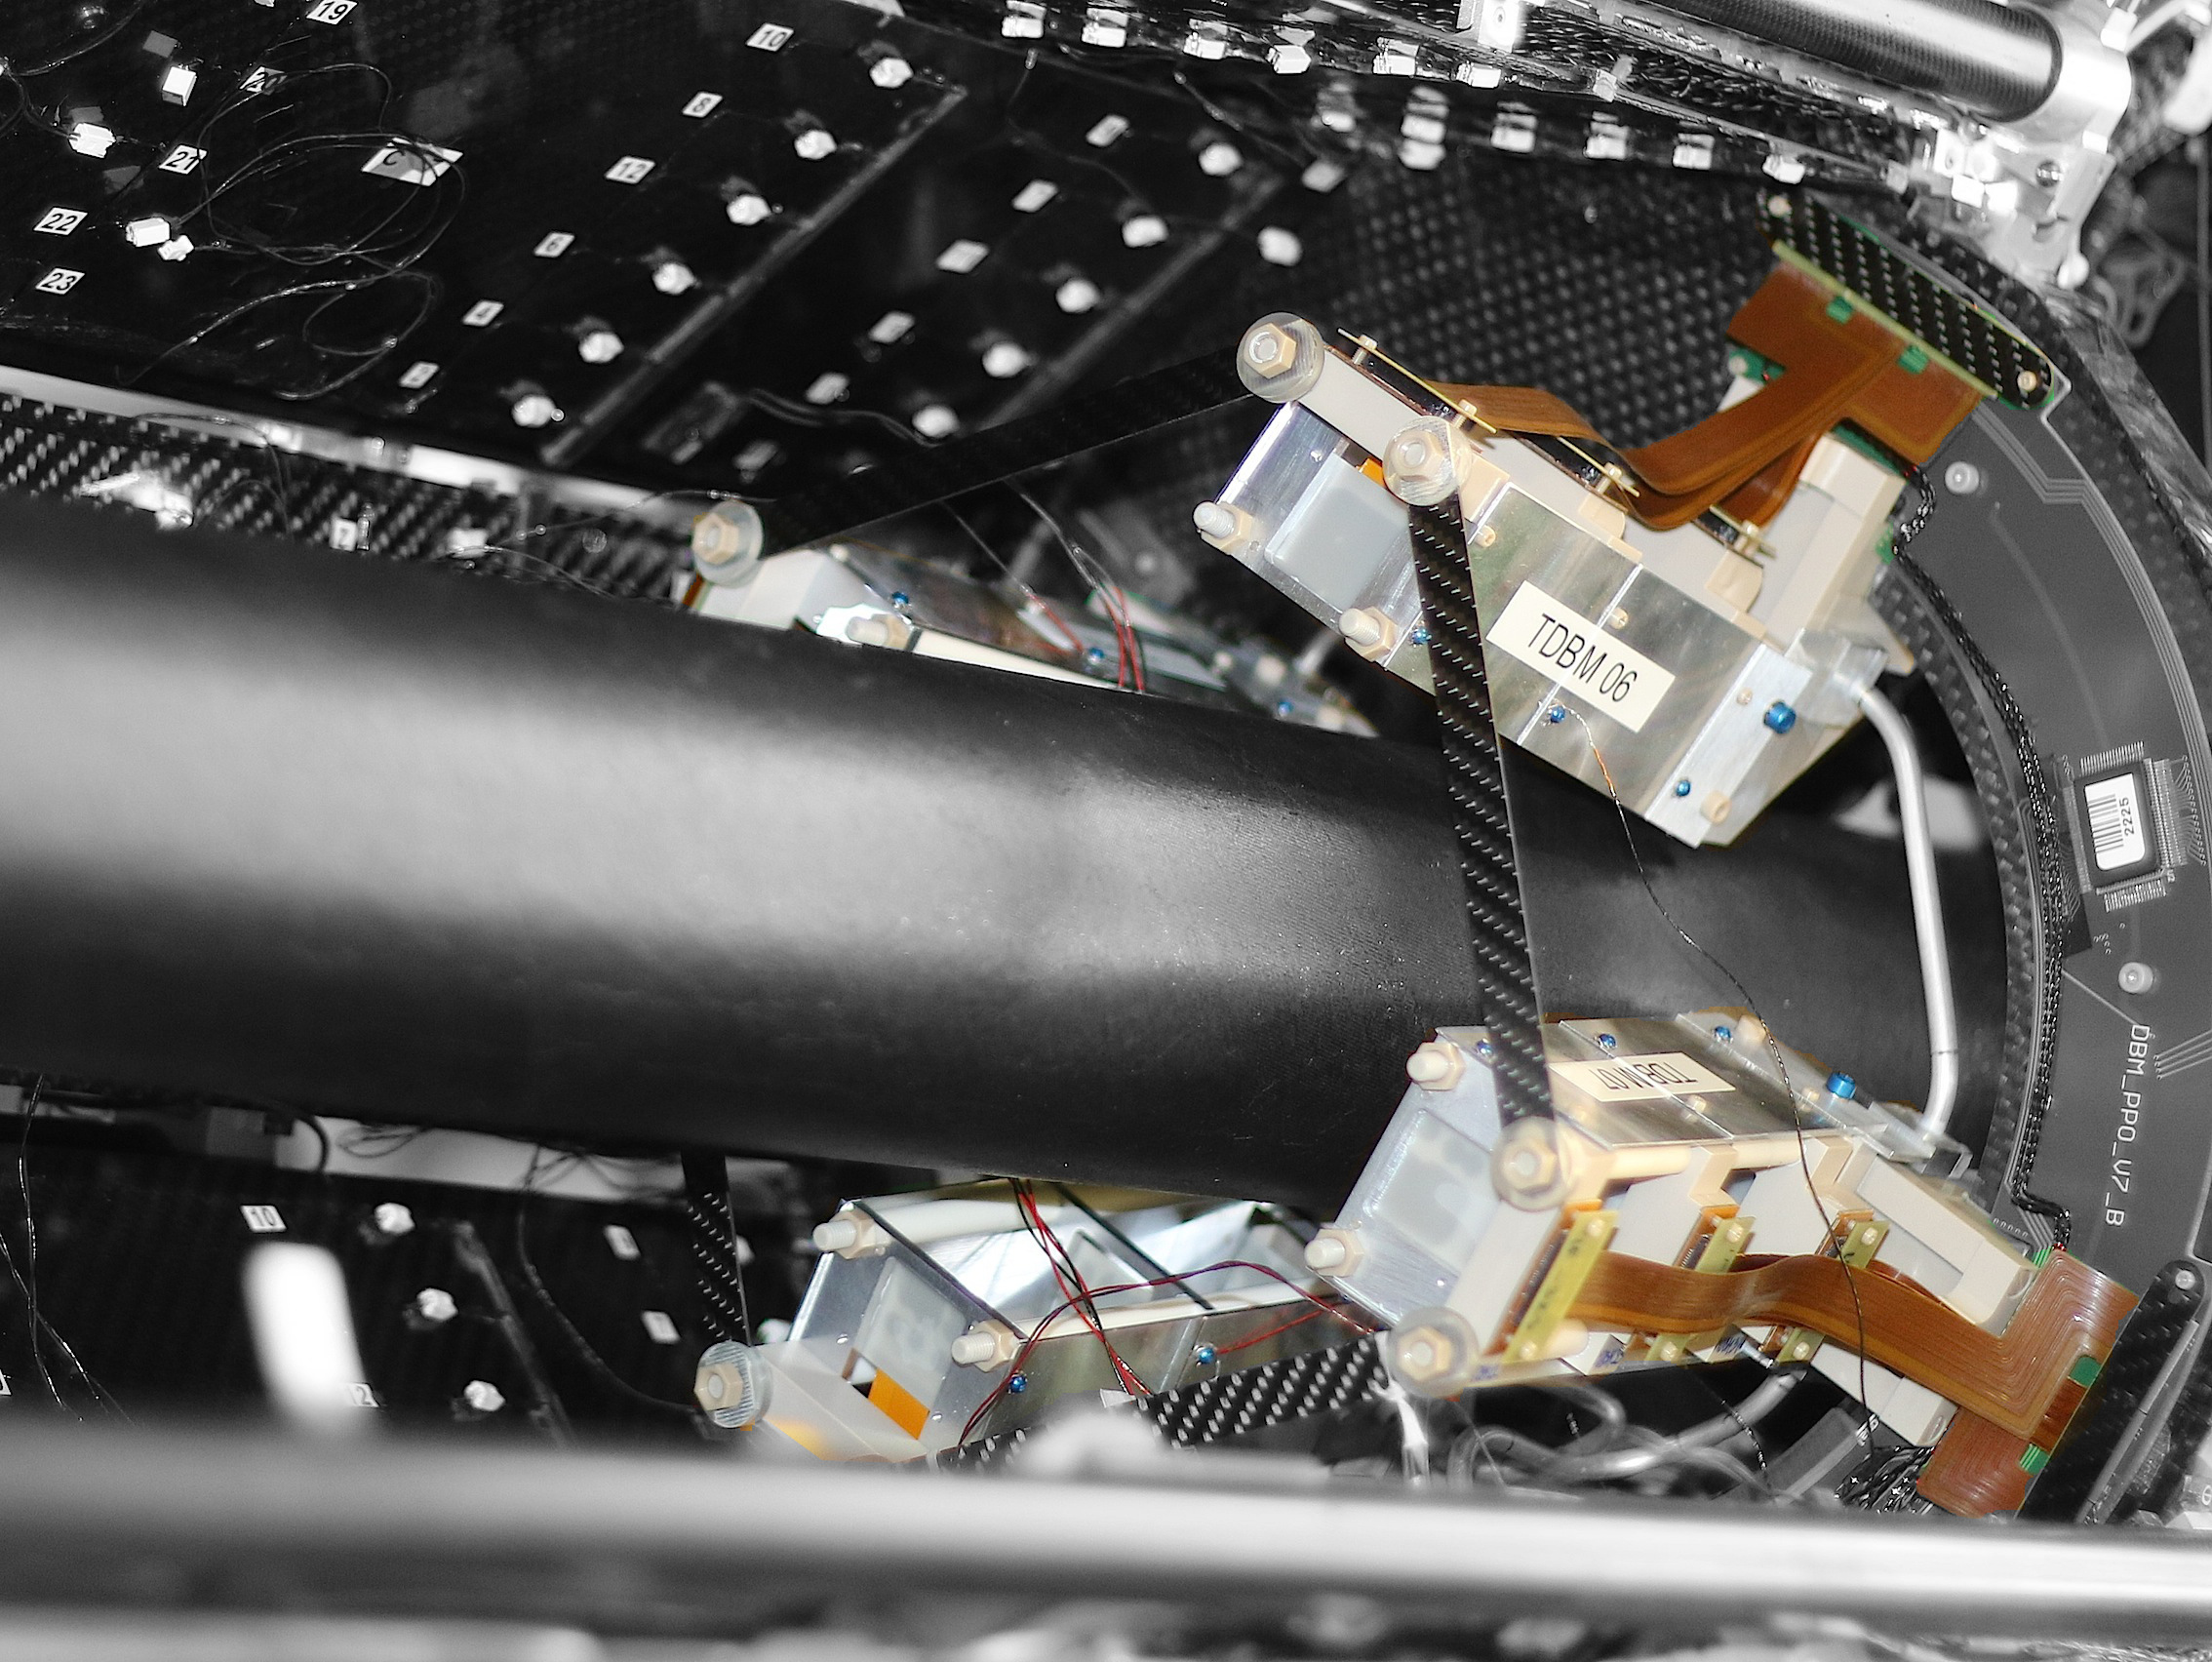
\includegraphics[width=0.7\textwidth]{04_charge_monitoring/pics/DBM-installed-colour1}
\caption{This photo highlights four telescopes installed onto the nSQPs and around the pipe.}
\label{fig:dbminatlas}
\end{figure}
For instance, if a strong magnetic field is applied perpendicular to the electric field lines in the diamond bulk, the leakage current stabilises. The DBM was designed to exploit this phenomenon. The magnetic field lines in the ATLAS experiment are parallel to the beam. Hence, an angular displacement of the sensor with respect to the beam allows for the leakage current suppression. However, the DBM telescopes still need to be directed towards the interaction region. Taking these considerations into account, a 10\textdegree~angle with respect to the beam pipe was chosen. The influence of the magnetic field on the particle tracks at this angle is very low as the field lines are almost parallel to the tracks. The tracks are therefore straight, which reduces the track reconstruction complexity.

\begin{figure}[!t]
\centering
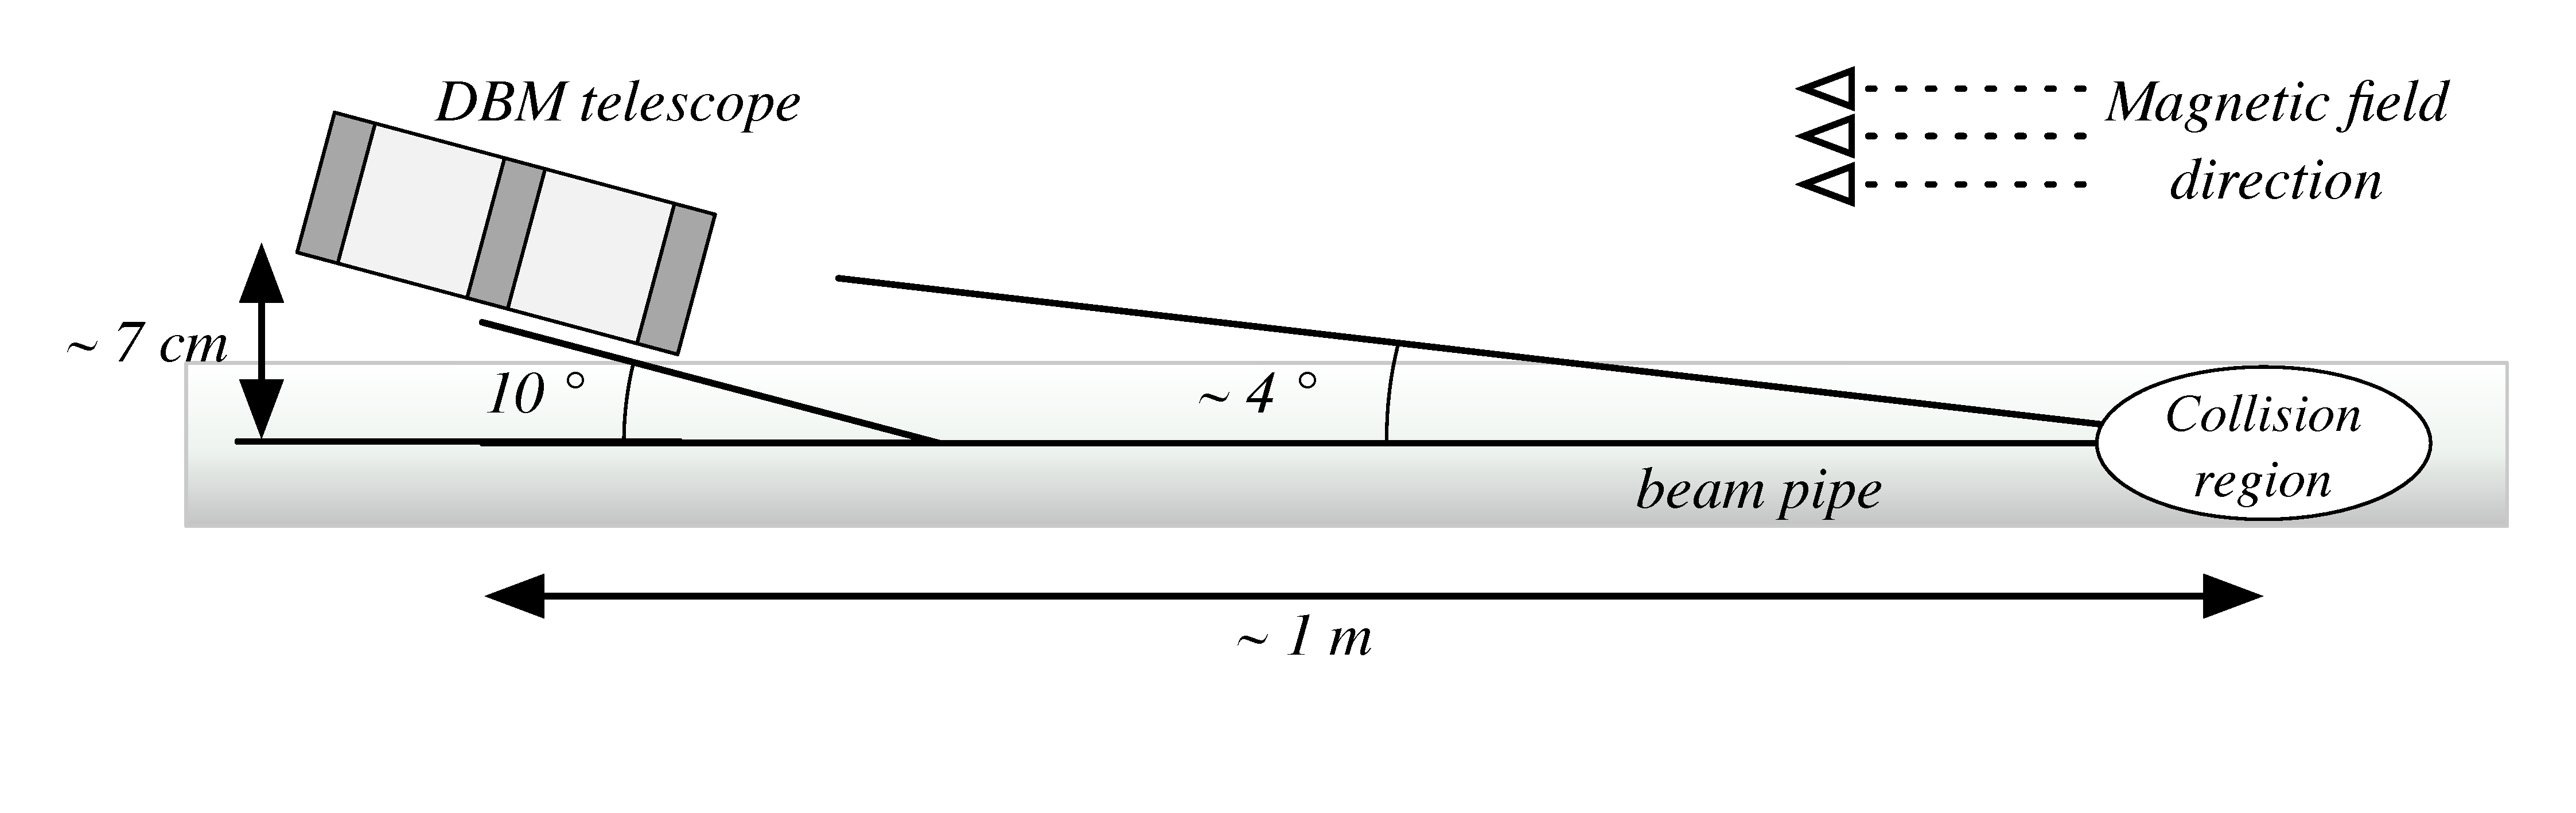
\includegraphics[width=0.7\textwidth]{../scripts/04_charge_monitoring/plots/DBM-positioning}
\caption{Position of the DBM in the ATLAS experiment.}
\label{fig:dbminatlas}
\end{figure}




%---------------------------------------------------------------------------------------------------------------
\section{Operation}
\label{sec:operation}
%---------------------------------------------------------------------------------------------------------------

The DBM has been commissioned in ATLAS and is now taking data. Several issues still need to be resolved regarding the readout system. Unfortunately, due to issues with the low voltage power supply regulators, six out of 24 modules were damaged during operation: four silicon and two diamond modules. The system configured the modules into an unsteady state whereby they drew twice as much current as the allowed maximum. This current most probably fused the wire bonds within minutes. This has left only five diamond telescopes fully operational. The preliminary data obtained using the remaining telescopes show that the background rejection could indeed work. 

The first step of the system test was to take data during collisions and check the occupancy in the individual modules. The occupancies were plotted side by side for comparison. Figure~\ref{fig:collocc} shows some of the occupancy values. At the time, the readout system was not yet configured to read out all telescopes in parallel. 
\begin{figure}[!t]
\centering
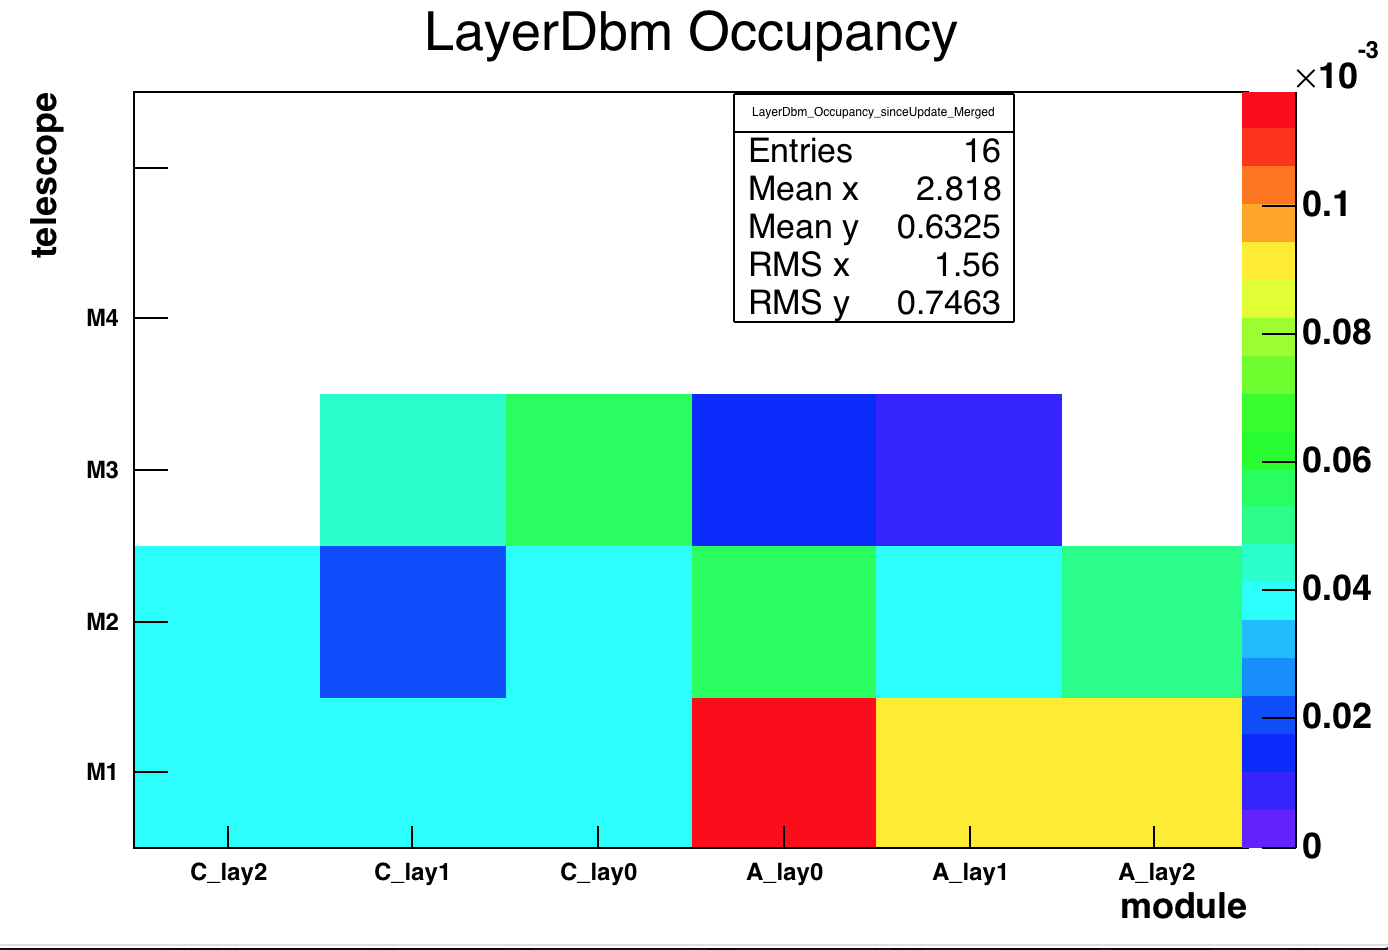
\includegraphics[width=0.7\textwidth]{04_charge_monitoring/pics/occupancy}
\caption{Occupancy of individual modules during collisions. Only 16 modules were taking data.}
\label{fig:collocc}
\end{figure}

The second step was to test the detector's capability of particle tracking. Only one telescope was used to take data with the beam. If all three planes of the telescope were hit during a bunch crossing, a linear line was fitted to the hits. This line represented the particle's trajectory. It was projected towards the interaction point. Two parameters were calculated where the line is the closest to the interaction point: the radial distance and the longitudinal distance between the line and the interaction point, as shown in figure~\ref{fig:z-r-distance}. This was done for the events with two colliding bunches as well as for events with only one, non-colliding bunch. The tracks recorded during the events with two colliding bunches could either come from the collisions or could the background scattering. Tracks recorded during a non-colliding bunch, on the other hand, are definitely background particles since there are no collisions taking place. 
\begin{figure}[!t]
\centering
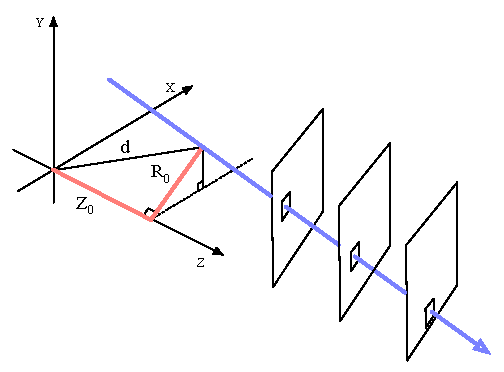
\includegraphics[width=0.7\textwidth]{../scripts/04_charge_monitoring/plots/z-r-distance}
\caption{A diagram showing the radial distance $R_\mathrm{0}$ and longitudinal distance $Z_\mathrm{0}$ of the trajectory from the interaction point at the minimal distance $d$. Z is the axis along the beam line. Three module planes intercept a particle and reconstruct its trajectory.}
\label{fig:z-r-distance}
\end{figure}

A comparison of the data acquired and depicted in figures~\ref{fig:raddist} and~\ref{fig:longdist} shows that, for the colliding bunches, the majority of the reconstructed tracks had the origin in the interaction point, with a narrow spread in $Z$ and $R$. For non-colliding bunches, the spread is wider. In the $Z_\mathrm{0}$ plot the distribution has one peak in the middle, which means that the empty RF buckets still held some particles which collided. The two peaks on the sides, however, show that a significant number of tracks had their origin at the radius of the beam pipe. Therefore these tracks were made by stray protons colliding with the beam pipe. These collisions are unwanted as they do not produce any meaningful physics while still damaging the ATLAS detector by means of the scattered radiation.

\begin{figure}[!t]
\centering
\begin{tabular}{cccc}
\subfloat{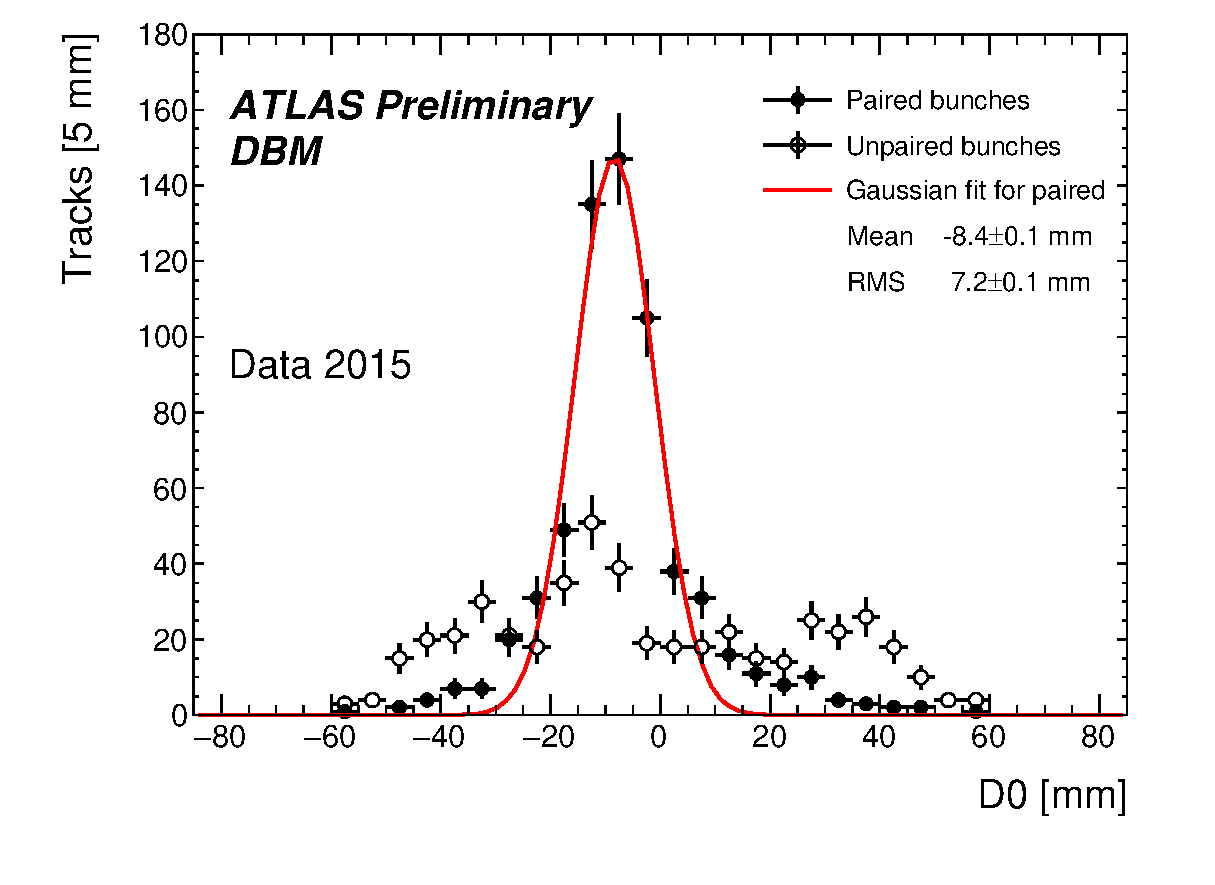
\includegraphics[width=0.7\textwidth]{../scripts/04_charge_monitoring/plots/D0} \label{fig:raddist}} \\
\subfloat{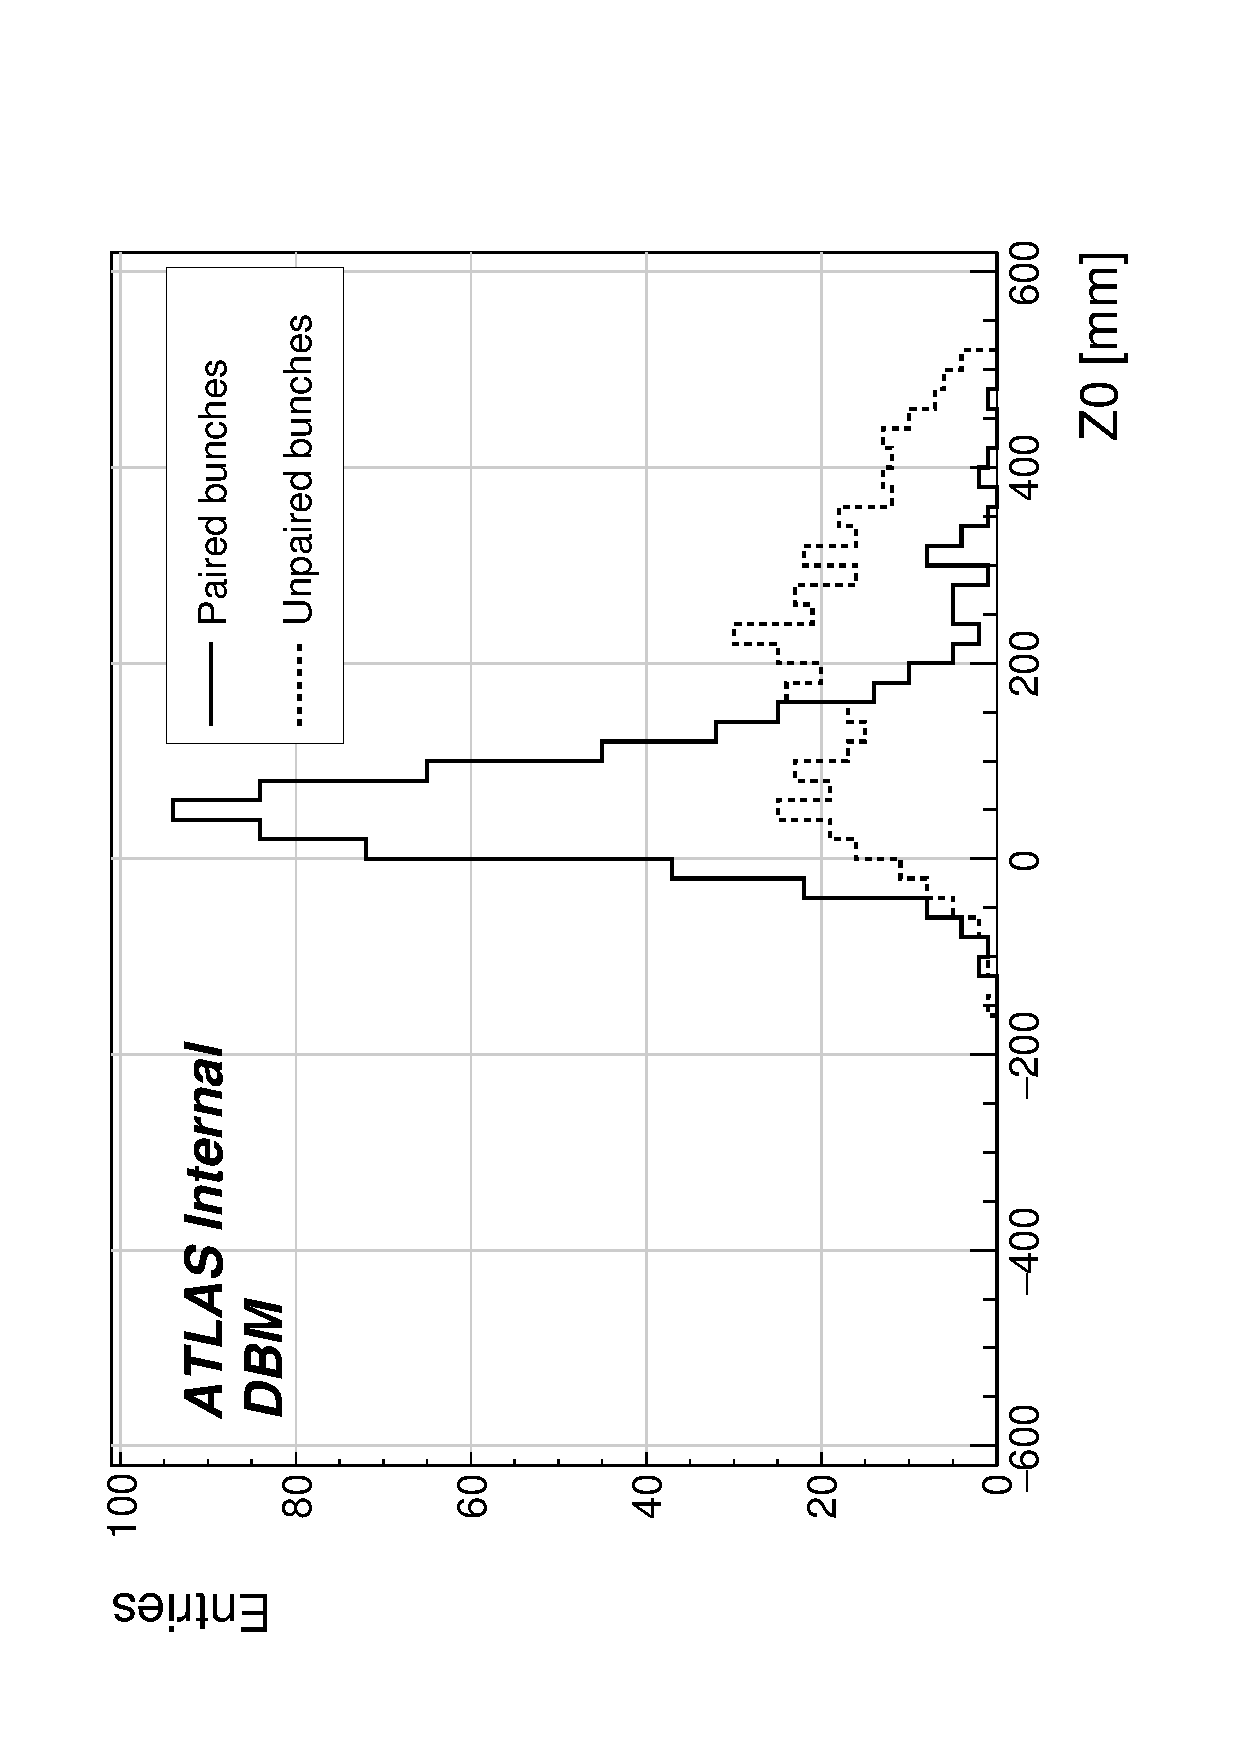
\includegraphics[width=0.7\textwidth]{../scripts/04_charge_monitoring/plots/Z0}  \label{fig:longdist}}
\end{tabular}
\caption{These two plots show two parameters of particle tracks recorded by one of the DBM telescopes: radial (a) and longitudinal (b) distance of the projected tracks from the interaction point.}
\end{figure}



%%---------------------------------------------------------------------------------------------------------------
%\section{Limitations}
%\label{sec:limitations}
%%---------------------------------------------------------------------------------------------------------------
%comparison between diamond and silicon modules

%---------------------------------------------------------------------------------------------------------------
\section{Conclusion}
\label{sec:limitations}
%---------------------------------------------------------------------------------------------------------------
The Diamond Beam Monitor has been designed as an upgrade to the existing luminosity detectors in the ATLAS experiment. It is the first diamond pixel tracking detector installed in a high-energy physics experiment. The pixelated front-end electronic chips ensure precise spatial detection of the charged high-energy particles. The projective geometry allows for particle tracking and background rejection. The detector is placed in a high-radiation forward region of the experiment. Therefore, radiation hardness of the chosen pCVD diamond sensors is an important requirement. The tests carried out in the test beam and in the laboratory confirmed that enough detector-grade DBM modules have been built to be installed in the experiment. The DBM is now running in ATLAS during collisions. Further improvements have to be made on the readout firmware before it is included in the main readout stream. 
